%----------------------------------------------------------------------------
% MediHaven project report. Formatting follows the SPIT ESE report template
% (synopsis.tex: 12 pt, A4, single-sided, margins 20/20/20/50 mm, numbered
% IEEE-style references) and the chapter structure of the Mini Project Report
% Preparation Guidelines (T.E. Computer Engineering, AY 2026-27).
% Build:  tectonic main.tex        (see README.md for alternatives)
%----------------------------------------------------------------------------
\documentclass[12pt,oneside,a4paper]{report}

\usepackage[T1]{fontenc}
\usepackage{lmodern}
\usepackage{geometry}
\geometry{left=20mm,right=20mm,top=20mm,bottom=50mm}
\usepackage{graphicx}
\usepackage{adjustbox}
\usepackage{xcolor}
\usepackage{amsmath,amssymb}
\usepackage{booktabs,tabularx,array,multirow,longtable}
\usepackage{caption}
\captionsetup{font=small,labelfont=bf}
\captionsetup[table]{position=top}
\usepackage{float}
\usepackage{enumitem}
\setlist{nosep,leftmargin=*}
\usepackage{tikz}
\usetikzlibrary{shapes.geometric,shapes.misc,shapes.multipart,arrows.meta,positioning,fit,calc,backgrounds,matrix}
\usepackage{pgfplots}
\pgfplotsset{compat=1.18}
\usepackage{url}
\usepackage{cite}
\usepackage{titlesec}
\usepackage{tocloft}
\setlength{\cftbeforechapskip}{4pt}
\setlength{\cftbeforesecskip}{0pt}
\setlength{\cftbeforefigskip}{1pt}
\setlength{\cftbeforetabskip}{1pt}
\renewcommand{\cftsecfont}{\small}
\renewcommand{\cftsecpagefont}{\small}
\usepackage[hidelinks]{hyperref}
\usepackage{algorithm}
\usepackage{algpseudocode}

% Compact chapter headings (keeps the report within the template's page range)
\titleformat{\chapter}[hang]{\bfseries\LARGE}{\thechapter\hspace{0.6em}}{0pt}{}
\titlespacing*{\chapter}{0pt}{0pt}{14pt}
\renewcommand{\arraystretch}{1.15}
\setcounter{tocdepth}{1}
% Let floats sit at the top/bottom of text pages instead of forcing gaps
\renewcommand{\topfraction}{0.9}
\renewcommand{\bottomfraction}{0.8}
\renewcommand{\textfraction}{0.07}
\renewcommand{\floatpagefraction}{0.85}
\setcounter{topnumber}{3}
\setcounter{totalnumber}{5}
\newcolumntype{Y}{>{\raggedright\arraybackslash}X}
\setlength{\parskip}{3pt}

% \bstctlcite (from IEEEtran.cls) so IEEEtran.bst options work with the report class
\makeatletter
\def\bstctlcite{\@ifnextchar[{\@bstctlcite}{\@bstctlcite[@auxout]}}
\def\@bstctlcite[#1]#2{\@bsphack\@for\@citeb:=#2\do{%
  \edef\@citeb{\expandafter\@firstofone\@citeb}%
  \if@filesw\immediate\write\csname #1\endcsname{\string\citation{\@citeb}}\fi}\@esphack}
\makeatother

% Code identifiers (test names, paths) that may break after underscores and slashes
\makeatletter
\g@addto@macro{\UrlBreaks}{\do\_\do\/\do\.}
\makeatother
\newcommand{\code}[1]{\nolinkurl{#1}}

% ============================================================================
% Project identity. Replace every \missing{...} with the verified value, then
% rebuild (see README.md). \missing renders a red marker so nothing unverified
% can slip into the submitted PDF unnoticed.
% ============================================================================
\newcommand{\missing}[1]{\textcolor{red}{\textbf{[#1]}}}

% Title used in the repository (README.md). Confirm it matches the approved title.
\newcommand{\ProjectTitle}{MediHaven: Integrated Multimodal Clinical Intelligence and Sovereign Medical Vault Platform}
\newcommand{\ProjectShortTitle}{MediHaven}
\newcommand{\GroupNumber}{\missing{Group No.}}

% Group members: first names verified from the repository; surnames and UIDs are not recorded there.
\newcommand{\StudentA}{Vidhi \missing{Surname}}
\newcommand{\StudentB}{Nirupam \missing{Surname}}
\newcommand{\StudentC}{Param \missing{Surname}}
\newcommand{\UIDA}{\missing{UID}}
\newcommand{\UIDB}{\missing{UID}}
\newcommand{\UIDC}{\missing{UID}}

\newcommand{\GuideName}{\missing{Guide name and designation}}
\newcommand{\HODName}{\missing{Head of Department name}}
\newcommand{\PrincipalName}{\missing{Principal name}}

% Course details: Report Preparation Guidelines (T.E. Computer Engineering, AY 2026--27) and README.md
\newcommand{\Programme}{Bachelor of Technology}
\newcommand{\Branch}{Computer Engineering}
\newcommand{\Department}{Department of Computer Engineering}
\newcommand{\CourseName}{T.E.\ Mini Project (Semester V)}
\newcommand{\AcademicYear}{2026--27}
\newcommand{\SubmissionMonth}{\missing{Month Year of submission}}

% Shared TikZ styles for all report and poster diagrams.
\definecolor{mhblue}{HTML}{0369A1}
\definecolor{mhteal}{HTML}{0F766E}
\definecolor{mhamber}{HTML}{B45309}
\definecolor{mhred}{HTML}{B91C1C}
\definecolor{mhgray}{HTML}{475569}
\definecolor{mhlight}{HTML}{F1F5F9}
\tikzset{
  >={Stealth[length=2.2mm]},
  box/.style={draw=mhgray, rounded corners=2pt, fill=white, align=center, font=\footnotesize,
              minimum height=7mm, inner sep=3pt},
  blue box/.style={box, draw=mhblue, fill=mhblue!8},
  teal box/.style={box, draw=mhteal, fill=mhteal!8},
  amber box/.style={box, draw=mhamber, fill=mhamber!10},
  red box/.style={box, draw=mhred, fill=mhred!7},
  layer/.style={draw=mhgray!60, dashed, rounded corners=4pt, inner sep=5pt},
  layer label/.style={font=\scriptsize\bfseries, text=mhgray, anchor=north west},
  flow/.style={->, draw=mhgray, thick},
  dflow/.style={->, draw=mhgray, thick, dashed},
  lbl/.style={font=\scriptsize, fill=white, inner sep=1pt},
  actor/.style={draw=mhgray, circle, minimum size=5mm, fill=mhlight},
  usecase/.style={draw=mhblue, ellipse, fill=mhblue!6, align=center, font=\scriptsize, inner sep=1.5pt,
                  minimum height=7mm},
  store/.style={draw=mhteal, fill=mhteal!8, font=\footnotesize, align=center, inner sep=3pt,
                minimum height=6mm, shape=rectangle, path picture={
                  \draw[mhteal] (path picture bounding box.north west) -- (path picture bounding box.north east);}},
  process/.style={draw=mhblue, fill=mhblue!8, circle, align=center, font=\scriptsize, inner sep=1pt,
                  minimum size=17mm},
  entity/.style={draw=mhgray, fill=white, align=left, font=\scriptsize, inner sep=2pt, rectangle split,
                 rectangle split parts=2, rectangle split part fill={mhblue!12, white}},
  state/.style={draw=mhblue, fill=mhblue!7, rounded corners=6pt, align=center, font=\footnotesize,
                minimum height=8mm, minimum width=22mm},
  decision/.style={draw=mhamber, fill=mhamber!10, diamond, aspect=2.2, align=center, font=\scriptsize,
                   inner sep=1pt},
  term/.style={draw=mhgray, fill=mhgray!15, rounded rectangle, align=center, font=\footnotesize,
               minimum height=6mm},
}


\begin{document}
\bstctlcite{IEEEexample:BSTcontrol}% IEEEtran: list at most 6 authors, else first 3 et al.

% ---------------- Preliminary pages (roman numbering) ----------------------
\pagenumbering{roman}
% Cover page adapted from the SPIT template (be_title.tex) for the Department of Computer Engineering.
\begin{titlepage}
\centering
\vspace*{0.2cm}
{\Large\textbf{\ProjectTitle}}\\[0.55cm]
submitted in partial fulfillment of the requirement\\
for the award of the Degree of\\[0.5cm]
{\large\textbf{\Programme}}\\
in\\
{\large\textbf{\Branch}}\\[0.25cm]
\CourseName\\[0.4cm]
by\\[0.4cm]
\begin{tabular}{ll}
{\large\textbf{\StudentA}} & UID: \UIDA\\
{\large\textbf{\StudentB}} & UID: \UIDB\\
{\large\textbf{\StudentC}} & UID: \UIDC\\
\end{tabular}\\[0.3cm]
Group No.: \GroupNumber\\[0.4cm]
under the guidance of\\[0.3cm]
{\large\textbf{\GuideName}}\\[0.4cm]

\includegraphics[scale=0.6]{figures/spitlogo.pdf}\\[0.3cm]
\textbf{\Department}\\
Bharatiya Vidya Bhavan's\\
Sardar Patel Institute of Technology\\
(Autonomous Institute Affiliated to University of Mumbai)\\
Munshi Nagar, Andheri-West, Mumbai-400058\\
University of Mumbai\\[0.2cm]
Academic Year \AcademicYear
\end{titlepage}

% Certificate in the format of the SPIT template (be_certificate1.tex). Signatures must be real:
% this page deliberately carries empty signature lines and no approval is implied until signed.
\clearpage
\thispagestyle{empty}
\vspace*{0.5cm}
\begin{center}
{\large\textbf{Certificate}}
\end{center}
\vspace{0.6cm}
This is to certify that the project entitled ``\ProjectTitle'' by \StudentA, \StudentB\ and \StudentC\
is submitted for the partial fulfillment of the \CourseName\ under the guidance of \GuideName\ for the
award of the Degree of \Programme\ in \Branch\ from the University of Mumbai.

\vspace{1.4cm}
\begin{center}\textbf{Certified by}\end{center}
\vspace{1.6cm}

\noindent\begin{tabular*}{\textwidth}{@{}l@{\extracolsep{\fill}}r@{}}
\rule{5.5cm}{0.4pt} & \rule{5.5cm}{0.4pt}\\
\textbf{\GuideName} & \textbf{\HODName}\\
Project Guide & Head of Department\\
\end{tabular*}

\vspace{1.8cm}
\begin{center}
\rule{5.5cm}{0.4pt}\\
\textbf{\PrincipalName}\\
Principal
\end{center}

\vfill
\begin{center}

\includegraphics[scale=0.55]{figures/spitlogo.pdf}\\[0.2cm]
\textbf{\Department}\\
Bharatiya Vidya Bhavan's Sardar Patel Institute of Technology\\
(Autonomous Institute Affiliated to University of Mumbai)\\
Munshi Nagar, Andheri (W), Mumbai-400058\\
\SubmissionMonth
\end{center}

% Approval certificate in the format of the SPIT template (be_certificate2.tex). To be signed by the
% examiners at evaluation; nothing on this page implies that approval has been given.
\clearpage
\thispagestyle{empty}
\vspace*{0.5cm}
\begin{center}
{\large\textbf{Approval Certificate}}
\end{center}
\vspace{1cm}
This is to certify that the project entitled ``\ProjectTitle'' by \StudentA, \StudentB\ and \StudentC\
is approved for the partial fulfillment of the \CourseName\ towards obtaining the Degree of \Programme\
in \Branch\ from the University of Mumbai.

\vspace{2.2cm}
\noindent\begin{tabular*}{\textwidth}{@{}l@{\extracolsep{\fill}}l@{}}
\textbf{Project Guide} & \textbf{External Examiner}\\[1.6cm]
\textbf{(signature)} & \textbf{(signature)}\\[0.8cm]
\textbf{Name:} & \textbf{Name:}\\[0.8cm]
\textbf{Date:} & \textbf{Date:}\\[1.8cm]
\textbf{Head of Department} & \textbf{Principal}\\
\end{tabular*}

\vspace{2cm}
\begin{center}
\textbf{Seal of the Institute}
\end{center}

% Declaration: wording from the SPIT template (synopsis.tex), extended with the truthful-reporting
% statement required by the Report Preparation Guidelines (Section 2.3). Signed by the students.
\clearpage
\thispagestyle{empty}
\vspace*{0.5cm}
\begin{center}
{\large\textbf{Declaration}}
\end{center}
\vspace{0.8cm}
We wish to state that the work embodied in this report titled ``\ProjectTitle'' forms our own
contribution to the work carried out under the guidance of \GuideName\ at the Sardar Patel Institute
of Technology. We declare that this written submission represents our ideas in our own words and
where others' ideas or words have been included, we have adequately cited and referenced the original
sources. We also declare that we have adhered to all principles of academic honesty and integrity and
have not misrepresented or fabricated or falsified any idea/data/fact/source in our submission.

We further declare that the implementation, test and evaluation results reported here are those
actually obtained from the project repository, that features are described as implemented only where
supporting evidence exists, and that MediHaven is an educational software prototype that has not been
clinically validated.

\vspace{2.5cm}
\noindent\begin{tabular*}{\textwidth}{@{}c@{\extracolsep{\fill}}c@{\extracolsep{\fill}}c@{}}
\rule{4.2cm}{0.4pt} & \rule{4.2cm}{0.4pt} & \rule{4.2cm}{0.4pt}\\
\textbf{\StudentA} & \textbf{\StudentB} & \textbf{\StudentC}\\
UID: \UIDA & UID: \UIDB & UID: \UIDC\\
\end{tabular*}

\vspace{1.5cm}
\noindent Date: \rule{3.5cm}{0.4pt}\hfill Place: Mumbai

\clearpage
\chapter*{Acknowledgement}
\addcontentsline{toc}{chapter}{Acknowledgement}
We express our sincere gratitude to our project guide, \GuideName, for guidance and feedback
throughout the development of this project, and to the Head of the \Department\ and the Principal of
Sardar Patel Institute of Technology for providing the facilities and academic environment in which this
work was carried out.

We thank the creators and maintainers of the MIMIC-IV Clinical Database Demo and PhysioNet for making
de-identified critical-care data openly available for research and teaching, and the developers of the
open-source software on which MediHaven is built, in particular Flask, scikit-learn, pandas, DuckDB and
Chart.js.

Finally, we thank our families and classmates for their support and encouragement.

\vspace{1.2cm}
\noindent\StudentA\hfill\StudentB\hfill\StudentC

\chapter*{Abstract}
\addcontentsline{toc}{chapter}{Abstract}
Clinical deterioration is often recognised late, patients seldom control who sees their records, and
published clinical machine-learning results are frequently hard to reproduce. MediHaven is an educational
software prototype that addresses these issues together in a single Flask web application. Physicians see
a triage dashboard in which a K-Means, decision-tree, k-nearest-neighbour and multilayer-perceptron
ensemble classifies synthetic inpatients into four risk tiers, with every model's vote, a decision-tree
rule path and similar historical cases. Patients keep a medical vault and share selected records through
HMAC-signed, expiring, scope- and use-limited QR passes whose redemption is atomic and audited. An
explicitly opt-in, loopback-only research mode rebuilds an in-hospital-mortality task from the MIMIC-IV
Clinical Database Demo (prediction at ICU admission + 24 hours) and serves only hash-verified artifacts.

Built with Python, Flask, SQLite, scikit-learn, DuckDB and Chart.js, the system applies database design,
concurrency control, algorithm analysis and software-engineering practice, and is tested by 354 automated
tests, all passing. Under a load test of the production server, a risk prediction took 71.9~ms (median,
one client), throughput saturated at about 15 predictions per second (CPU-bound), simple reads reached
268.8 requests per second at 16 clients, there were no errors, and memory stayed below 210~MB.

On the 107 eligible ICU stays (11 deaths), patient-grouped five-fold cross-validation gave pooled AUROCs of
0.74 (logistic regression), 0.73 (random forest), 0.77 (neural network) and 0.56 (smoothed decision tree),
with 95\,\% intervals spanning roughly 0.35--0.91, and results changed markedly when four outcome-timestamp
anomalies were removed. By contrast, the synthetic ensemble scored 1.00 on a 20-patient hold-out, which
reflects the data generator rather than clinical skill. MediHaven therefore demonstrates an honest,
reproducible engineering pipeline; it is not clinically validated and must not be used for patient care.

\vspace{0.4cm}
\noindent\textbf{Keywords:} clinical decision support, early warning, explainable machine learning,
MIMIC-IV, grouped cross-validation, patient-controlled records, QR access, Flask.

\clearpage
\tableofcontents
\clearpage
\listoffigures
\clearpage
\listoftables
\clearpage
\chapter*{List of Abbreviations and Symbols}
\addcontentsline{toc}{chapter}{List of Abbreviations and Symbols}
\begin{small}
\begin{tabularx}{\textwidth}{@{}lY@{\hspace{1.2em}}lY@{}}
\toprule
API & Application Programming Interface & KPI & Key Performance Indicator\\
AP & Average Precision & LLM & Large Language Model\\
AUROC & Area Under the Receiver Operating Characteristic curve & MAP & Mean Arterial Pressure\\
BP & Blood Pressure (SBP systolic, DBP diastolic) & MIMIC & Medical Information Mart for Intensive Care\\
BUN & Blood Urea Nitrogen & MLP & Multilayer Perceptron\\
CI & Confidence Interval & OOF & Out-of-Fold (prediction)\\
CSP & Content Security Policy & OLS & Ordinary Least Squares\\
CV & Cross-Validation & PHR & Personal Health Record\\
DFD & Data Flow Diagram & QR & Quick Response (code)\\
EHR & Electronic Health Record & RBAC & Role-Based Access Control\\
ER & Entity--Relationship & REST & Representational State Transfer\\
FR / NFR & Functional / Non-Functional Requirement & SpO$_2$ & Peripheral oxygen saturation\\
HMAC & Hash-based Message Authentication Code & SQL & Structured Query Language\\
HR & Heart Rate & SRS & Software Requirements Specification\\
ICU & Intensive Care Unit & TLS & Transport Layer Security\\
JWT & JSON Web Token & UML & Unified Modeling Language\\
KNN & $k$-Nearest Neighbours & WAL & Write-Ahead Logging (SQLite)\\
\midrule
$p$ & cohort death rate (prevalence) & $\hat{y}$ & predicted probability of the positive class\\
$n,\,d$ & number of samples, number of features & $k$ & number of neighbours / clusters / folds\\
\bottomrule
\end{tabularx}
\end{small}


% ---------------- Main chapters (arabic numbering) --------------------------
\clearpage
\pagenumbering{arabic}
\chapter{Introduction and Problem Definition}
\label{ch:intro}

\section{Project Background}
Hospital wards generate a continuous stream of vital signs and laboratory results, yet deterioration is
still often recognised late. Track-and-trigger scores such as the National Early Warning Score (NEWS)
\cite{smith2013news} and severity scores such as SAPS~II \cite{legall1993sapsii} reduce physiology to a
few thresholds, while machine-learning (ML) models trained on electronic health records (EHRs) report
higher discrimination \cite{rajkomar2018scalable,purushotham2018benchmarking}. At the same time, patients
rarely control who sees their own records, and clinicians who receive a patient from another facility
must often work without the history.

MediHaven is a web application, developed as a \CourseName\ in the \Department, that brings three
strands together in one teaching-scale system: (i) a physician triage dashboard that ranks synthetic
inpatients with four classical ML models and explains each vote, (ii) a patient-controlled medical vault
from which time-limited, scope-limited QR access passes can be shared, and (iii) an explicitly opt-in
research mode that rebuilds a real mortality-prediction task from the openly available MIMIC-IV Clinical
Database Demo \cite{johnson2023mimicivdemo,johnson2023mimiciv} and evaluates baselines with
leakage-aware, patient-grouped cross-validation.

MediHaven is an \textbf{educational software prototype}. It is not a medical device, it has not been
clinically validated, and none of its outputs may be used for diagnosis, treatment or other patient-care
decisions.

\section{Problem Statement}
Build a single, secure, testable web platform that (a) demonstrates explainable multi-model risk
stratification on realistic but synthetic inpatient data, (b) lets a patient grant a clinician
revocable, auditable and scope-restricted access to selected records, and (c) shows, on genuine
de-identified ICU data, how a mortality-risk pipeline must be built and evaluated honestly---without
leakage, with uncertainty, and without exposing patient-level data beyond the researcher's machine.

Existing approaches make this difficult: published models rarely release reproducible cohorts
\cite{johnson2017reproducibility}, deployed proprietary scores can perform far worse than reported
\cite{wong2021epicsepsis}, and record-sharing systems are typically institution-centred rather than
patient-controlled \cite{azaria2016medrec}.

\section{Motivation}
The project gives three groups something concrete: students and teachers obtain an end-to-end example
of clinical ML engineering (data pipeline, models, evaluation, serving, security and testing);
clinicians and evaluators can see how model votes, rule paths and uncertainty are presented; and
patients see a model of consent-based sharing with a visible access log. The research mode in
particular demonstrates the gap between an impressive demo accuracy on synthetic data and the much
more modest, uncertain performance obtained on real data (Chapter~\ref{ch:results}).

\section{Objectives}
\begin{enumerate}[label=O\arabic*.]
\item Implement role-based web portals for physicians, patients and administrators over a REST API.
\item Train and serve a four-model ensemble (K-Means, decision tree, KNN, MLP) that returns a risk tier,
      a score, per-model votes and an explanation for each synthetic patient.
\item Implement a patient vault with HMAC-signed, expiring, scope- and use-limited QR passes, an
      atomic use quota and an immutable access log.
\item Build a versioned MIMIC-IV Demo task (in-hospital mortality after the first 24 ICU hours) with
      explicit cohort, label and leakage rules, and evaluate baselines with patient-grouped
      cross-validation and bootstrap confidence intervals.
\item Serve verified research artifacts in a loopback-only research mode with integrity checks.
\item Protect secrets and data: strong-secret enforcement, CSP, rate limits, de-identified prompts
      to external AI, and no external AI in research mode.
\item Verify the system with an automated test suite and measure server performance under load.
\end{enumerate}

\section{Scope of the Project}
\textbf{Included:} the features above; a synthetic cohort of 100 patients; the MIMIC-IV Demo~2.2
(100 patients, 140 ICU stays); a production entry point (Waitress) and container recipe.
\textbf{Excluded:} real hospital integration (HL7/FHIR feeds), credentialed full MIMIC-IV, clinical
validation, real file uploads to the vault, and multi-instance deployment.
\textbf{Intended users:} students, teachers and evaluators; the physician/patient/administrator roles are
demonstration roles. \textbf{Operating environment:} Python~3.12 on Windows or Linux, a modern browser,
SQLite. \textbf{Expected scale:} a single server process serving tens of concurrent users
(Chapter~\ref{ch:scal}).

\section{Proposed Solution}
A layered Flask application (Chapter~\ref{ch:design}) serves Jinja2/JavaScript portals and a JSON API.
Synthetic predictions come from an in-memory ensemble whose weighted soft votes are fused into one of
four tiers; a decision-tree rule path and $k$ nearest historical cases make each result inspectable.
The vault issues HS256 JSON Web Tokens \cite{rfc7519} (HMAC \cite{rfc2104}) whose server-side record
holds the authoritative scope, expiry and use count. A separate research pipeline builds a hashed,
versioned dataset from MIMIC-IV Demo files outside the repository, trains five pipelines under grouped
cross-validation, and the web application serves only artifacts whose SHA-256 hashes verify.

\section{Novelty and Originality}
The individual algorithms are standard; the contribution is the \emph{integration and the engineering
discipline}: (i) one prototype combines explainable triage, patient-controlled sharing and a research
pipeline; (ii) research mode is fail-closed---it refuses unsafe secrets, non-loopback binding and
tampered artifacts, never falls back to synthetic data and never calls an external AI service;
(iii) the stay-level research view scores every ICU stay with an out-of-fold model and refuses to serve
unless the recomputed predictions reproduce the verified run exactly; and (iv) timestamp anomalies in the
outcome data are kept, flagged and analysed rather than silently dropped.

\section{Feasibility Analysis}
\textbf{Technical:} all components use mature open-source libraries (Flask, scikit-learn
\cite{pedregosa2011scikit}, pandas, DuckDB) and run on a laptop.
\textbf{Economic:} no licence costs; the MIMIC-IV Demo is open access; Gemini use is optional.
\textbf{Operational:} one command starts the demo (\texttt{run\_demo.py}); the production entry point
seeds and trains on first start. \textbf{Time and resources:} the repository history shows development
between 6 and 26 October 2026 (Section~\ref{sec:git}).

\section{Social Relevance and Practical Applications}
MediHaven is a teaching and demonstration artefact: it illustrates early-warning dashboards, consent-based
record sharing and responsible evaluation of clinical ML. Its practical value lies in education and in
prototyping user interfaces and data-protection patterns, not in patient care.

\section{Success Criteria and Key Performance Indicators}
Table~\ref{tab:kpi} lists the KPIs fixed for this project; Chapter~\ref{ch:testing} compares them with
the measured values.

\begin{table}[!htbp]
\centering
\caption{Key performance indicators and targets}
\label{tab:kpi}
\small
\begin{tabularx}{\textwidth}{@{}p{34mm}Yp{22mm}Y@{}}
\toprule
KPI & Definition & Target & Measurement method\\
\midrule
Functional correctness & passed / total automated tests & 100\,\% & \texttt{pytest} on the full suite\\
Response time & median latency of a risk prediction, 1 client & $\le$ 150 ms & timed HTTP requests to Waitress\\
Reliability & failed requests under 16 concurrent clients & 0 & 3{,}200-request load test\\
Throughput & simple API requests per second, 16 clients & $\ge$ 100 req/s & load test, \texttt{/api/vitals}\\
Resource use & server working set under load & $\le$ 512 MB & process-tree memory sampling\\
Synthetic model quality & hold-out accuracy on the synthetic split & $\ge$ 0.91 & project benchmark report\\
Research evaluation & discrimination with honest uncertainty & report AUROC with 95\% CI & grouped CV + bootstrap\\
\bottomrule
\end{tabularx}
\end{table}

\section{Organisation of the Report}
Chapter~\ref{ch:lit} reviews related systems and literature; Chapter~\ref{ch:srs} specifies requirements;
Chapter~\ref{ch:design} presents the architecture and design; Chapter~\ref{ch:algo} covers algorithms and
complexity; Chapter~\ref{ch:subjects} maps the work to the curriculum; Chapter~\ref{ch:impl} describes the
implementation; Chapters~\ref{ch:scal}--\ref{ch:results} report performance, testing and results; and
Chapter~\ref{ch:concl} concludes.

\chapter{Literature Review and Study of Existing Systems}
\label{ch:lit}

\section{Study of Existing Systems}
\textbf{Bedside scores.} NEWS aggregates vital-sign thresholds into an early-warning score
\cite{smith2013news}; SAPS~II estimates ICU mortality from 17 variables \cite{legall1993sapsii}. Both are
transparent and cheap but coarse. \textbf{Proprietary EHR-embedded models} such as the Epic Sepsis Model
are widely deployed, yet external validation can reveal much weaker performance than expected
\cite{wong2021epicsepsis}. \textbf{Research benchmarks} built on MIMIC
\cite{harutyunyan2019multitask,purushotham2018benchmarking} standardise tasks but are not applications.
\textbf{Patient-controlled sharing} prototypes such as MedRec use a blockchain for permissions
\cite{azaria2016medrec}. \textbf{LLM-based documentation} tools summarise clinical text
\cite{vanveen2024adapted}, with recognised factuality and safety risks \cite{singhal2023llmclinical}.

\section{Review of Research Papers and Technical Resources}
Eighteen peer-reviewed papers were reviewed; bibliographic details were verified against DOI, Crossref,
PubMed, PMLR or JMLR records. Findings are quoted only from the published abstracts.

\paragraph{[P1] MIMIC-IV \cite{johnson2023mimiciv}.} \emph{Problem:} hospital data are archived for
storage, not research. \emph{Approach:} a de-identified EHR database from Beth Israel Deaconess Medical
Center. \emph{Limitation:} single centre. \emph{Relation:} source of the demo subset used here
\cite{johnson2023mimicivdemo}, distributed via PhysioNet \cite{goldberger2000physionet}.

\paragraph{[P2] Harutyunyan et al.\ \cite{harutyunyan2019multitask}.} Four MIMIC-III benchmarks
(mortality, length of stay, physiologic decline, phenotyping) with linear and neural baselines and multitask
training. \emph{Limitation:} one database. \emph{Relation:} motivates MediHaven's fixed, versioned task
definition.

\paragraph{[P3] Purushotham et al.\ \cite{purushotham2018benchmarking}.} Deep models compared with a
Super Learner and SAPS~II/SOFA on MIMIC-III; deep models performed best, especially on raw time series.
\emph{Relation:} explains why a small tabular baseline set is a deliberate, modest starting point.

\paragraph{[P4] Rajkomar et al.\ \cite{rajkomar2018scalable}.} Deep models on whole EHRs in FHIR format
(216{,}221 inpatients, two centres) reported AUROC 0.93--0.94 for in-hospital mortality.
\emph{Limitation:} large, hard-to-interpret models and two centres. \emph{Relation:} an upper reference
point; MediHaven's demo cohort is three orders of magnitude smaller.

\paragraph{[P5] Johnson, Pollard and Mark \cite{johnson2017reproducibility}.} Reproducing 28 MIMIC
mortality studies found that half differed in sample size by more than 25\,\%. \emph{Relation:} MediHaven
publishes exact cohort, label and exclusion rules with counts for every step.

\paragraph{[P6] Pirracchio et al.\ (SICULA) \cite{pirracchio2015sicula}.} A Super Learner on MIMIC-II
(24{,}508 patients) achieved cross-validated AUROC 0.85--0.88 versus 0.78 for SAPS~II.
\emph{Limitation:} external validation on only 200 patients. \emph{Relation:} ensemble learning and
cross-validation, applied here at teaching scale.

\paragraph{[P7] SAPS II \cite{legall1993sapsii}.} 17 variables, 13{,}152 patients from 137 ICUs; AUROC
0.88 (development) and 0.86 (validation). \emph{Relation:} conceptual ancestor of the 24-hour
physiological summaries used as features.

\paragraph{[P8] NEWS \cite{smith2013news}.} NEWS discriminated the combined 24-hour outcome with AUROC
0.873 against 0.736--0.834 for 33 other scores. \emph{Limitation:} retrospective, one hospital.
\emph{Relation:} the synthetic dashboard's tiered early-warning presentation.

\paragraph{[P9] Wong et al.\ \cite{wong2021epicsepsis}.} External validation of the Epic Sepsis Model on
38{,}455 hospitalisations: AUROC 0.63; it missed 67\,\% of sepsis cases while alerting on 18\,\% of
patients. \emph{Relation:} the reason MediHaven reports uncertainty and refuses clinical claims.

\paragraph{[P10] TRIPOD \cite{collins2015tripod}.} A 22-item reporting checklist for prediction models.
\emph{Relation:} guided what the research mode reports (population, outcome, predictors, validation).

\paragraph{[P11] Kaufman et al.\ \cite{kaufman2012leakage}.} Formal definition of leakage and
``learn--predict separation''. \emph{Relation:} the forbidden-feature guard, the 24-hour window with
storetime checks and fold-internal preprocessing.

\paragraph{[P12] Saito and Rehmsmeier \cite{saito2015precision}.} On imbalanced data,
precision--recall plots reflect performance better than ROC plots. \emph{Relation:} average precision is
reported beside AUROC (prevalence 10.3\,\%).

\paragraph{[P13] Van Calster et al.\ \cite{vancalster2019calibration}.} Poor calibration misleads clinical
decisions; calibration curves need large samples. \emph{Relation:} Brier scores are reported, and
calibration is left as future work given 11 deaths.

\paragraph{[P14] Rudin \cite{rudin2019stop}.} Argues for inherently interpretable models in high-stakes
settings (position paper). \emph{Relation:} decision-tree rule paths and logistic coefficients are shown.

\paragraph{[P15] Sendak et al.\ \cite{sendak2020modelfacts}.} Proposes a one-page ``Model Facts'' label
telling clinicians how and when (not) to use a model. \emph{Relation:} the research page's model card and
disclaimers.

\paragraph{[P16] Azaria et al.\ (MedRec) \cite{azaria2016medrec}.} Blockchain-based record access and
permission management leaving data in providers' storage. \emph{Limitation:} prototype, not field
tested. \emph{Relation:} MediHaven pursues patient-controlled access with simpler signed, expiring tokens.

\paragraph{[P17] Van Veen et al.\ \cite{vanveen2024adapted}.} Adapted LLMs on four summarisation tasks;
physicians rated the best summaries equivalent (45\,\%) or superior (36\,\%) to experts, with an analysis
of fabricated content. \emph{Relation:} motivates optional, de-identified narrative synthesis.

\paragraph{[P18] Singhal et al.\ \cite{singhal2023llmclinical}.} MultiMedQA and human evaluation; Flan-PaLM
reached 67.6\,\% on MedQA but showed key gaps, and Med-PaLM remained inferior to clinicians.
\emph{Relation:} narratives are labelled as non-advice and never receive identifiers.

\section{Comparative Analysis}
\begin{table}[!htbp]
\centering
\caption{Comparison of existing approaches with MediHaven}
\label{tab:compare}
\small
\begin{tabularx}{\textwidth}{@{}lYYYY@{}}
\toprule
Criterion & Bedside scores \cite{smith2013news,legall1993sapsii} & Proprietary EHR models \cite{wong2021epicsepsis} & Research benchmarks \cite{harutyunyan2019multitask} & MediHaven\\
\midrule
Explainability & high (thresholds) & low & varies & rule path, votes, coefficients\\
Reproducibility & high & low (closed) & high & versioned, hashed artifacts\\
Uncertainty reported & rarely & rarely & sometimes & bootstrap 95\% CI\\
Patient-controlled sharing & no & no & no & QR passes with audit log\\
Clinical validation & yes & yes & n/a & \textbf{none} (prototype)\\
Cost & free & licensed & free & free / open source\\
\bottomrule
\end{tabularx}
\end{table}

\section{Limitations of Existing Systems}
Threshold scores are coarse; black-box models are hard to audit and may underperform on new sites
\cite{wong2021epicsepsis}; published cohorts are hard to reproduce \cite{johnson2017reproducibility};
leakage can inflate results \cite{kaufman2012leakage}; record sharing is rarely patient-controlled; and
LLM outputs can fabricate content \cite{vanveen2024adapted}.

\section{Identified Engineering Gap}
For teaching, no single open example combines explainable triage, consent-based sharing and an honest,
leakage-aware evaluation on real de-identified ICU data with fail-closed serving. This is an engineering
and educational gap, not a claim of a new clinical method.

\section{Proposed Improvements}
MediHaven addresses the gap with an integrated prototype whose research results are reproducible,
uncertainty-aware and explicitly limited; Chapter~\ref{ch:results} compares it with these systems.

\chapter{Software Requirements Specification (SRS)}
\label{ch:srs}

\section{Purpose and Scope of the SRS}
This SRS specifies the behaviour implemented in the MediHaven repository (branch \texttt{param}, October
2026). Requirements marked \emph{future} are not implemented.

\section{Intended Users and Stakeholders}
Physicians (triage, charts, QR scanning), patients (vault, sharing, access log), administrators (census,
reassignment, escalation, model telemetry), researchers (opt-in research mode on their own machine), and
evaluators/teachers. Demonstration accounts exist for each role; production deployments must replace
them (Section~\ref{sec:secdesign}).

\section{Overall Product Description}
A Python/Flask server with a SQLite database serves browser portals and a JSON API. Synthetic mode is the
default. Research mode is enabled only by \texttt{DATA\_MODE=mimic}, runs on loopback only, and reads
verified artifacts stored outside the repository. Optional dependency: the Google Gemini API (synthetic
mode only).

\section{Functional Requirements}
\begin{small}
\begin{longtable}{@{}p{12mm}p{48mm}p{44mm}p{56mm}@{}}
\caption{Functional requirements}\label{tab:fr}\\
\toprule
ID & Requirement (input $\rightarrow$ output) & Processing & Acceptance criterion\\
\midrule
\endfirsthead
\toprule ID & Requirement & Processing & Acceptance criterion\\ \midrule
\endhead
FR-01 & Sign in with username/password $\rightarrow$ session and role dashboard & hash check, rate limit & wrong password 401; 11th attempt in 5 min returns 429\\
FR-02 & Role-based access to portals and APIs & session role vs route & patient cannot read another patient (403)\\
FR-03 & Triage roster with tiers and filters & DB query, latest prediction & 100 synthetic patients listed with tiers\\
FR-04 & Patient chart: tier, score, 4 model votes, vitals, rule path, similar cases & ensemble inference & every patient returns 4 votes; 72-h chart non-empty\\
FR-05 & Alert feed, acknowledgement, escalation dispatch & in-memory alert state & identity taken from the signed-in user\\
FR-06 & Vault records: add and list by category & category whitelist & invalid category 422\\
FR-07 & Share QR pass with scope, lifetime, uses & HS256 JWT + DB record & lifetime $\le$ 30 days, uses $\le$ 1000\\
FR-08 & Redeem pass by token or image & signature, expiry, revocation, atomic quota & single-use pass granted once under 4 concurrent scans\\
FR-09 & Revoke pass; view access log & ownership check & revoked pass is denied and logged\\
FR-10 & Clinical narrative (handover/discharge) & de-identified Gemini prompt or local fallback & no identifier in the prompt\\
FR-11 & Research: model card, dashboard, what-if estimate & verified artifacts only & forbidden/invalid inputs rejected (422)\\
FR-12 & Research triage: all ICU stays with out-of-fold scores & recompute and verify OOF & mismatch with saved metrics gives 503\\
FR-13 & Health endpoint & model and mode status & \texttt{GET /api/health} returns 200\\
\bottomrule
\end{longtable}
\end{small}

\section{Non-Functional Requirements}
\begin{table}[!htbp]
\centering
\caption{Non-functional requirements}
\label{tab:nfr}
\small
\begin{tabularx}{\textwidth}{@{}lY@{}}
\toprule
Category & Requirement (implemented)\\
\midrule
Performance & median prediction latency $\le$ 150 ms for one client; simple reads $\ge$ 100 req/s\\
Scalability & one process, thread pool of 8; documented single-instance limit (Chapter~\ref{ch:scal})\\
Reliability & fail-closed research serving; first-start bootstrap reseeds an empty or interrupted database\\
Security/privacy & strong secrets enforced off-loopback; hashed passwords; CSP and security headers; 8-hour sessions; no MIMIC identifiers in responses or logs; research mode never calls external AI\\
Usability & consistent dark clinical theme; keyboard \textsc{Esc} closes dialogs; responsive header below 900 px\\
Maintainability & modular blueprints and services; 354 automated tests; pinned dependencies\\
Portability & Windows and Linux; Docker image recipe (Python 3.12)\\
Resource use & server working set $\le$ 512 MB; database about 1.2 MB, model files about 0.2 MB\\
\bottomrule
\end{tabularx}
\end{table}

\section{Hardware and Software Requirements}
\textbf{Hardware (measured on):} Intel Core i5-8250U (4 cores, 8 threads), 7.9 GB RAM, Windows 11.
Minimum: 2 cores, 2 GB RAM, 1 GB disk. \textbf{Software:} Python 3.12; Flask 3.1, Werkzeug 3.1, Waitress
3.0.2; pandas 3.0, NumPy 2.5, SciPy 1.18, scikit-learn 1.9.1, joblib 1.6; DuckDB 1.5 and PyArrow 26
(research); PyJWT 2.15, qrcode 8.2, Pillow 12.3, OpenCV (headless) 5.0, pyzbar 0.1.9 (optional);
pytest 9.1; Chart.js 4.4.1 (self-hosted). All versions are pinned in \texttt{requirements.txt}.

\section{Constraints and Assumptions}
\begin{itemize}
\item \textbf{Data:} only synthetic patients in the web demo; MIMIC-IV Demo data stay outside the
      repository and OneDrive and are never sent to external services (data use terms).
\item \textbf{Technical:} SQLite and in-process state imply a single server instance; research
      artifacts are tied to the exact scikit-learn version used for training.
\item \textbf{Time/cost:} one academic semester; free and open-source tools only.
\item \textbf{Assumption:} evaluators run the system locally or on one small server with HTTPS.
\end{itemize}

\section{Use Cases and User Stories}
Figure~\ref{fig:usecase} summarises the use cases by role.
\begin{figure}[!htbp]
\centering
\adjustbox{max width=0.85\linewidth}{% Use-case diagram (roles from src/api/auth.py; use cases from the routes and portal guards).
\begin{tikzpicture}[x=1mm, y=1mm]
\newcommand{\stick}[3]{% x, y, label
  \draw[mhgray, thick] (#1,#2+5) circle (2.2);
  \draw[mhgray, thick] (#1,#2+2.8) -- (#1,#2-2.5) (#1-3.5,#2+1) -- (#1+3.5,#2+1)
        (#1,#2-2.5) -- (#1-3,#2-7) (#1,#2-2.5) -- (#1+3,#2-7);
  \node[font=\footnotesize\bfseries, below] at (#1,#2-7.5) {#3};}
\draw[mhgray, rounded corners=4pt] (24,51) rectangle (150,-54);
\node[font=\footnotesize\bfseries, anchor=north west] at (26,50) {MediHaven};
\stick{8}{15}{Physician}
\stick{8}{-33}{Patient}
\stick{166}{3}{Administrator}
% physician
\node[usecase] (u2) at (55,27) {View triage roster\\and risk tiers};
\node[usecase] (u3) at (55,15) {Open patient chart\\(4 model votes, vitals)};
\node[usecase] (u10) at (55,3) {Research triage \&\\what-if (opt-in mode)};
% shared
\node[usecase] (u1) at (55,-10) {Sign in};
\node[usecase] (u4) at (110,44) {Scan QR access pass};
% patient
\node[usecase] (u5) at (55,-24) {Manage vault records};
\node[usecase] (u6) at (55,-35) {Share / revoke QR pass};
\node[usecase] (u7) at (55,-46) {View own access log};
% administrator
\node[usecase] (u8) at (122,12) {Reassign patient,\\dispatch escalation};
\node[usecase] (u9) at (122,-20) {Model telemetry,\\Gemini synthesis};
\foreach \u in {u2,u3,u10,u1} \draw[mhgray] (12,16) -- (\u.west);
\draw[mhgray] (8,22.5) -- (u4.west);
\foreach \u in {u1,u5,u6,u7} \draw[mhgray] (12,-32) -- (\u.west);
\foreach \u in {u8,u9,u1} \draw[mhgray] (162,4) -- (\u.east);
\draw[mhgray] (164,8) -- (u4.east);
\end{tikzpicture}
}
\caption{Use-case diagram}
\label{fig:usecase}
\end{figure}
\noindent Representative user stories: \emph{As a physician}, I open a critical patient's chart and see
why each model voted as it did. \emph{As a patient}, I share only my allergies and medications for one
hour with a single-use pass and later see who used it. \emph{As a researcher}, I see each ICU stay's
out-of-fold risk next to its actual outcome without any MIMIC identifier leaving my computer.

\chapter{System Architecture and Design}
\label{ch:design}

\section{Overall System Architecture}
MediHaven follows a layered client--server architecture (Figure~\ref{fig:arch}). The browser renders
server-side Jinja2 templates and calls the JSON API with \texttt{fetch}; the Flask application factory
(\code{src/api/app.py}) wires security middleware and six blueprints; services hold the ML models, the
vault logic, the narrative synthesiser and the research service; SQLite, model files and the research
artifacts form the data layer.

\begin{figure}[!htbp]
\centering
\adjustbox{max width=\linewidth}{% Overall layered architecture (verified against src/api/app.py, routes/, models/, vault/, training/).
% Explicit millimetre grid: 6 columns in the upper layers, 4 in the lower layers.
\begin{tikzpicture}[x=1mm, y=1mm]
\newcommand{\band}[3]{% top y, bottom y, title
  \draw[mhgray!60, dashed, rounded corners=3pt] (0,#1) rectangle (170,#2);
  \node[layer label] at (1.5,#1-0.8) {#3};}
\band{0}{-19}{Presentation: Jinja2 templates, JavaScript, Chart.js (browser)}
\foreach \x/\t in {15/Landing \& Login, 43/Physician Triage, 71/Patient Vault, 99/QR Scanner,
                   127/Admin Overview, 155/Research (opt-in)}
  \node[blue box, minimum width=25mm, text width=23mm] at (\x,-11.5) {\t};

\band{-25}{-58}{Application: Flask app factory served by Waitress (wsgi.py) or run\_demo.py}
\node[teal box, minimum width=164mm] at (85,-36)
  {session RBAC $\cdot$ CSP and security headers $\cdot$ rate limits $\cdot$ research-mode boundary $\cdot$ JSON error handlers};
\foreach \x/\t in {15/auth, 43/patients, 71/predictions, 99/alerts, 127/vault, 155/research}
  \node[teal box, minimum width=25mm] at (\x,-49.5) {/api/\t};

\band{-64}{-86}{Services}
\node[amber box, minimum width=38mm, text width=35mm] (ens) at (22,-76.5) {4-model ensemble\\K-Means $\cdot$ DT $\cdot$ KNN $\cdot$ MLP};
\node[amber box, minimum width=38mm, text width=35mm] (qr) at (64,-76.5) {Vault \& QR service\\HMAC-signed JWT passes};
\node[amber box, minimum width=38mm, text width=35mm] (nlp) at (106,-76.5) {Narrative synthesiser\\de-identified prompts};
\node[amber box, minimum width=38mm, text width=35mm] (rs) at (148,-76.5) {Research service\\verified artifacts};

\band{-92}{-114}{Data and external services}
\node[store, minimum width=38mm, text width=35mm] (ms) at (22,-104.5) {models\_store/\\joblib model files};
\node[store, minimum width=38mm, text width=35mm] (db) at (64,-104.5) {SQLite (WAL mode)\\8 tables, 8 indexes};
\node[store, minimum width=38mm, text width=35mm] (gm) at (106,-104.5) {Google Gemini API\\external, optional};
\node[store, minimum width=38mm, text width=35mm] (ra) at (148,-104.5) {Research artifacts\\outside repo \& OneDrive};

\draw[flow] (85,-19) -- node[lbl, right=1mm]{HTTP + JSON (fetch), session cookie} (85,-25);
\draw[flow] (85,-58) -- (85,-64);
\draw[flow] (ens.south) -- (ms.north);
\draw[flow] (ens.south east) -- (db.north west);
\draw[flow] (qr.south) -- (db.north);
\draw[dflow] (nlp.south) -- node[lbl, right]{synthetic mode only} (gm.north);
\draw[flow] (rs.south) -- node[lbl, right]{hash-verified} (ra.north);
\end{tikzpicture}
}
\caption{Layered architecture of MediHaven}
\label{fig:arch}
\end{figure}

\section{Component and Module Description}
\begin{table}[!htbp]
\centering
\caption{Major modules: purpose, inputs, outputs and dependencies}
\label{tab:modules}
\small
\begin{tabularx}{\textwidth}{@{}p{40mm}YYp{30mm}@{}}
\toprule
Module & Purpose & Input $\rightarrow$ output & Depends on\\
\midrule
\code{api/app.py}, \texttt{auth.py} & app factory, RBAC, headers, rate limits & HTTP request $\rightarrow$ routed response & config, security\\
\texttt{routes/patients, predictions, alerts} & triage and charts & patient id $\rightarrow$ JSON packet & ensemble, SQLite\\
\code{models/ensemble.py} + 4 models & synthetic risk inference & 30 features $\rightarrow$ tier, score, votes & scikit-learn\\
\code{vault/*}, \code{routes/vault} & records, QR passes, audit & scope, token $\rightarrow$ scoped records & PyJWT, OpenCV\\
\code{nlp/summarizer.py} & narratives & coarse model outputs $\rightarrow$ text & Gemini API (optional)\\
\code{tasks/build_mimic_t1.py} & research dataset & MIMIC CSV $\rightarrow$ hashed parquet & DuckDB, pandas\\
\code{training/*} & research training, verification, serving & dataset $\rightarrow$ verified run, OOF view & scikit-learn\\
\texttt{bootstrap.py}, \texttt{wsgi.py} & first start, production entry & config $\rightarrow$ ready app & Waitress\\
\bottomrule
\end{tabularx}
\end{table}

\section{Architecture Selection and Justification}
A layered, modular monolith was chosen over microservices: the workload is small (Chapter~\ref{ch:scal}),
the team is three students, models load once into process memory (no network hop per prediction), and a
single SQLite file keeps deployment trivial. Blueprints and service classes keep the layers separable, so
the data layer or the model service could later be extracted.

\section{Data Flow Diagrams}
Figure~\ref{fig:dfd0} shows the context and Figure~\ref{fig:dfd1} the level-1 processes and stores. The
Gemini flow is dashed because it is optional and only ever receives coarse model outputs.

\begin{figure}[!htbp]
\centering
\adjustbox{max width=0.85\linewidth}{% Context-level (level 0) DFD: one process, external entities, labelled flows.
\begin{tikzpicture}[x=1mm, y=1mm]
\node[process, minimum size=26mm, font=\footnotesize] (sys) at (85,0) {\textbf{0}\\MediHaven\\system};
\node[box, minimum width=28mm] (phys) at (14,24) {Physician};
\node[box, minimum width=28mm] (pat) at (14,-24) {Patient};
\node[box, minimum width=28mm] (adm) at (156,24) {Administrator};
\node[box, minimum width=28mm] (gem) at (156,-24) {Google Gemini API\\(synthetic mode only)};
\node[box, minimum width=40mm] (mimic) at (85,-38) {MIMIC-IV Demo files\\(offline research build)};
% each actor: request flow above, response flow below
\draw[flow] ($(phys.east)+(0,1.5)$) -- node[lbl, above, sloped, pos=0.45]{credentials, chart requests, QR scans} (sys.130);
\draw[flow] (sys.155) -- node[lbl, below, sloped, pos=0.55]{tiers, charts, vault records} ($(phys.east)+(0,-1.5)$);
\draw[flow] ($(pat.east)+(0,-1.5)$) -- node[lbl, below, sloped, pos=0.45]{records, share scope} (sys.230);
\draw[flow] (sys.205) -- node[lbl, above, sloped, pos=0.55]{QR pass, access log} ($(pat.east)+(0,1.5)$);
\draw[flow] ($(adm.west)+(0,1.5)$) -- node[lbl, above, sloped, pos=0.45]{reassign, dispatch} (sys.50);
\draw[flow] (sys.25) -- node[lbl, below, sloped, pos=0.55]{census, model telemetry} ($(adm.west)+(0,-1.5)$);
\draw[dflow] (sys.335) -- node[lbl, above, sloped, pos=0.55]{de-identified prompt} ($(gem.west)+(0,1.5)$);
\draw[dflow] ($(gem.west)+(0,-1.5)$) -- node[lbl, below, sloped, pos=0.35]{narrative text} (sys.310);
\draw[flow] (mimic.north) -- node[lbl, left]{stay-level features} (sys.south);
\end{tikzpicture}
}
\caption{Context-level (level-0) data flow diagram}
\label{fig:dfd0}
\end{figure}

\begin{figure}[!htbp]
\centering
\adjustbox{max width=0.88\linewidth}{% Level-1 DFD: processes 1.0-5.0, data stores D1-D3 and external entities.
\begin{tikzpicture}[x=1mm, y=1mm]
\node[box, minimum width=24mm] (user) at (10,0) {Physician /\\Patient /\\Admin};
\node[process] (p1) at (48,24) {\textbf{1.0}\\Authenticate\\\& authorise};
\node[process] (p2) at (48,-24) {\textbf{2.0}\\Triage \&\\predict};
\node[process] (p3) at (98,24) {\textbf{3.0}\\Vault \&\\QR sharing};
\node[store, minimum width=30mm] (d1) at (98,0) {D1\;SQLite database};
\node[process] (p4) at (98,-24) {\textbf{4.0}\\Narrative\\synthesis};
\node[store, minimum width=30mm] (d2) at (10,-42) {D2\;models\_store};
\node[box, minimum width=24mm] (ext) at (98,-48) {Gemini API};
\node[process] (p5) at (150,-12) {\textbf{5.0}\\Research\\pipeline};
\node[store, minimum width=32mm] (d3) at (150,18) {D3\;research artifacts};
\node[box, minimum width=28mm] (mim) at (150,-42) {MIMIC-IV Demo};
\draw[flow] (user) -- node[lbl, above, sloped]{credentials} (p1);
\draw[flow] (user) -- node[lbl, below, sloped]{chart request} (p2);
\draw[flow] (p1) -- node[lbl, left]{session role} (p2);
\draw[flow] (p1) -- node[lbl, above]{session role} (p3);
\draw[flow] (p3) -- node[lbl, right]{tokens, access log} (d1);
\draw[flow] (d1) -- node[lbl, above, sloped]{vitals, labs} (p2);
\draw[flow] (d2) -- node[lbl, below, sloped]{fitted models} (p2);
\draw[flow] (p2) -- node[lbl, below]{risk packet} (p4);
\draw[dflow] (p4) -- node[lbl, right]{coarse outputs only} (ext);
\draw[flow] (mim) -- node[lbl, right]{CSV} (p5);
\draw[flow] (p5) -- node[lbl, right]{verified run} (d3);
\end{tikzpicture}
}
\caption{Level-1 data flow diagram}
\label{fig:dfd1}
\end{figure}

\section{UML Diagrams}
The use-case diagram appears in Figure~\ref{fig:usecase}. Figure~\ref{fig:class} shows the main classes:
the ensemble aggregates four model wrappers, and the research service composes the verified artifacts and
the lazily built stay view. Figure~\ref{fig:seq} traces the redemption of a QR pass; the use count is
claimed with a single conditional \texttt{UPDATE}, so concurrent scans cannot overspend a pass.
Figure~\ref{fig:activity} gives the activity flow of a prediction, Figure~\ref{fig:state} the life cycle
of a pass, and Figure~\ref{fig:deploy} the deployment options.

\begin{figure}[!htbp]
\centering
\adjustbox{max width=\linewidth}{% Class diagram of the main model and service classes (names and members from the source code).
\begin{tikzpicture}[x=1mm, y=1mm,
  cls/.style={draw=mhgray, fill=white, rectangle split, rectangle split parts=3, align=left,
              font=\scriptsize, inner sep=2pt, text width=#1, rectangle split part fill={mhblue!12,white,white}},
  cls/.default=40mm]
\node[cls=58mm] (ens) at (85,32) {\textbf{EnsembleClinicalPredictor}
  \nodepart{second} weights: dict (DT .30, MLP .30, KNN .25, K-Means .15)\\ scaler: StandardScaler
  \nodepart{third} train\_from\_data() / load()\\ predict\_patient(id): dict};
\node[cls=39mm] (km) at (18,4) {\textbf{KMeansRiskClustering}
  \nodepart{second} n\_clusters = 4\\ cluster\_to\_tier\_code
  \nodepart{third} fit(), predict\_proba()};
\node[cls=39mm] (dt) at (62,4) {\textbf{DecisionTreeRiskClassifier}
  \nodepart{second} max\_depth = 5
  \nodepart{third} fit(), predict(), explain()};
\node[cls=39mm] (knn) at (106,4) {\textbf{KNNSimilarityMatcher}
  \nodepart{second} n\_neighbors = 5
  \nodepart{third} find\_similar(), recommend\_protocol()};
\node[cls=39mm] (nn) at (150,4) {\textbf{NeuralNetworkRiskModel}
  \nodepart{second} hidden\_layer\_sizes = (64, 32)
  \nodepart{third} fit(), predict\_proba()};
\foreach \c in {km,dt,knn,nn} \draw[mhgray, -{Diamond[open,length=3mm]}] (\c.north) -- (ens.south);

\node[cls=48mm] (rms) at (30,-30) {\textbf{ResearchModelService}
  \nodepart{second} artifacts: VerifiedArtifacts\\ stays: LazyStayView
  \nodepart{third} status(), dashboard(), predict()\\ stay\_roster(), stay\_detail(n)};
\node[cls=40mm] (va) at (88,-30) {\textbf{VerifiedArtifacts}
  \nodepart{second} run\_manifest, metrics\\ features (74), models
  \nodepart{third} verify\_and\_load(dir, pin)};
\node[cls=38mm] (lsv) at (145,-30) {\textbf{LazyStayView}
  \nodepart{second} lock, cached view or error
  \nodepart{third} get(): StayView};
\node[cls=44mm] (sdt) at (88,-58) {\textbf{SmoothedDecisionTree}
  \nodepart{second} max\_depth 3, min leaf 8, $m = 5$\\ leaf\_rate\_ (m-estimate)
  \nodepart{third} fit(), predict\_proba()};
\node[cls=48mm] (sum) at (30,-58) {\textbf{ClinicalNarrativeSummarizer}
  \nodepart{second} GEMINI\_MODELS, api\_key
  \nodepart{third} generate(), external\_calls\_allowed()};
\draw[mhgray, -{Diamond[length=3mm]}] (va.west) -- (rms.east);
\draw[mhgray, -{Diamond[length=3mm]}] (lsv.north west) to[bend right=12] (rms.north east);
\draw[dflow] (va.south) -- node[lbl, right]{loads pipeline using} (sdt.north);
\end{tikzpicture}
}
\caption{Class diagram of the model and service layer}
\label{fig:class}
\end{figure}

\begin{figure}[!htbp]
\centering
\adjustbox{max width=\linewidth}{% Sequence diagram: clinician redeems a QR access pass (src/api/routes/vault.py, src/vault/*).
\begin{tikzpicture}[x=1mm, y=1mm]
\foreach \x/\n/\t in {8/c/Clinician browser, 44/r/vault route (POST), 82/a/access\_controller,
                      118/s/qr\_scanner, 152/d/SQLite}
  {\node[box, minimum width=28mm, text width=26mm] (\n) at (\x,0) {\t};
   \draw[mhgray, dashed] (\x,-4) -- (\x,-80);}
\newcommand{\msg}[5][]{\draw[flow,#1] (#2,#4) -- node[lbl, above]{#5} (#3,#4);}
\msg{8}{44}{-10}{token or image (session cookie)}
\node[lbl, right, align=left, font=\scriptsize\itshape] at (45,-17) {RBAC, payload type check,\\signed-in user = auditor};
\msg{44}{82}{-24}{access\_vault\_with\_token()}
\msg{82}{118}{-30}{scan\_and\_validate\_qr()}
\msg{118}{152}{-36}{token by hash: revoked? expiry? uses?}
\msg[dflow]{152}{118}{-42}{token record}
\node[lbl, align=center] at (135,-48) {HMAC-SHA256 JWT check\\(signature, expiry)};
\msg[dflow]{118}{82}{-54}{valid / reason}
\msg{82}{152}{-60}{atomic UPDATE use\_count (if uses remain)}
\msg{82}{152}{-66}{INSERT vault\_access\_log}
\msg[dflow]{82}{44}{-72}{scoped records}
\msg[dflow]{44}{8}{-78}{200 JSON or 403 reason}
\end{tikzpicture}
}
\caption{Sequence diagram: redeeming a QR access pass}
\label{fig:seq}
\end{figure}

\begin{figure}[!htbp]
\centering
\adjustbox{max width=0.75\linewidth}{% Activity diagram: synthetic risk prediction (predictions.py -> ensemble.predict_patient).
\begin{tikzpicture}[node distance=5mm, act/.style={box, text width=100mm, font=\footnotesize}]
\node[term] (s) {start: GET /api/patients/\{id\}/predict};
\node[decision, below=of s] (auth) {session role\\physician or admin?};
\node[act, below=of auth] (load) {load vitals, labs and medications from SQLite; engineer 30 features (latest values,\\72-hour means and OLS slopes, shock index, MAP)};
\node[act, below=of load] (scale) {scale the feature vector with the stored StandardScaler};
\node[act, below=of scale] (four) {K-Means, decision tree, KNN and MLP each return a 4-tier probability vector};
\node[act, below=of four] (fuse) {fuse: $p = 0.30\,p_{DT} + 0.30\,p_{MLP} + 0.25\,p_{KNN} + 0.15\,p_{KM}$; tier $= \arg\max_t p_t$;\\score $= \sum_t p_t s_t$ with $s = (0.10, 0.45, 0.78, 0.94)$};
\node[act, below=of fuse] (save) {store a prediction row; return tier, score, per-model votes, rule path and similar cases};
\node[term, below=of save] (e) {end: 200 JSON};
\node[term, fill=mhred!12, right=14mm of auth] (deny) {401 / 403};
\node[term, fill=mhred!12, right=6mm of scale.east, anchor=west, yshift=-6mm] (fail) {500, generic message};
\draw[flow] (s) -- (auth);
\draw[flow] (auth) -- node[lbl, right]{yes} (load);
\draw[flow] (auth) -- node[lbl, above]{no} (deny);
\draw[flow] (load) -- (scale); \draw[flow] (scale) -- (four); \draw[flow] (four) -- (fuse);
\draw[flow] (fuse) -- (save); \draw[flow] (save) -- (e);
\draw[dflow] (four.east) -| node[lbl, below, pos=0.25]{model error} (fail.south);
\end{tikzpicture}
}
\caption{Activity diagram: synthetic risk prediction}
\label{fig:activity}
\end{figure}

\begin{figure}[!htbp]
\centering
\adjustbox{max width=0.85\linewidth}{% State machine of a QR access pass (qr_generator.py, qr_scanner.py, access_controller.py).
\begin{tikzpicture}[x=1mm, y=1mm]
\fill[mhgray] (0,0) circle (1.6);
\node[state] (act) at (34,0) {Active\\\scriptsize use\_count $<$ max\_uses};
\node[state] (used) at (100,14) {Exhausted\\\scriptsize use\_count = max\_uses};
\node[state] (exp) at (100,0) {Expired\\\scriptsize now $>$ expires\_at};
\node[state] (rev) at (100,-14) {Revoked\\\scriptsize by the patient};
\draw[flow] (1.6,0) -- node[lbl, above]{share (patient)} (act);
\draw[flow] (act) to[loop above] node[lbl, above]{granted scan: atomic use\_count + 1} (act);
\draw[flow] (act) -- node[lbl, above, sloped]{last allowed scan} (used);
\draw[flow] (act) -- node[lbl, above]{TTL elapses ($\le$ 30 days)} (exp);
\draw[flow] (act) -- node[lbl, below, sloped]{revoke} (rev);
\node[font=\scriptsize, align=left, anchor=west] at (122,0) {terminal: every further\\scan is denied and\\written to the access log};
\end{tikzpicture}
}
\caption{State machine of a QR access pass}
\label{fig:state}
\end{figure}

\begin{figure}[!htbp]
\centering
\adjustbox{max width=\linewidth}{% Deployment diagram: public synthetic deployment vs local-only research mode (wsgi.py, Dockerfile, run_demo.py).
\begin{tikzpicture}[x=1mm, y=1mm]
\node[box, minimum width=24mm] (user) at (12,12) {Browser\\(HTTPS)};
\node[box, minimum width=24mm, text width=22mm] (proxy) at (12,-12) {TLS reverse\\proxy};
\draw[mhblue, rounded corners=4pt, thick] (28,30) rectangle (104,-30);
\node[font=\scriptsize\bfseries, text=mhblue, anchor=north west, text width=72mm] at (29.5,29) {Server or container (synthetic demo, production mode)};
\node[teal box, text width=30mm] (w) at (48,12) {Waitress, 8 threads\\wsgi.py $\rightarrow$ Flask};
\node[amber box, text width=26mm] (b) at (87,12) {src.bootstrap:\\seed, train if missing};
\node[store, text width=30mm] (db) at (48,-14) {SQLite volume\\/app/database};
\node[store, text width=26mm] (ms) at (87,-14) {models\_store,\\data/processed};
\draw[flow] (user) -- (proxy); \draw[flow] (proxy.east) -- (w.south west);
\draw[flow] (w) -- (db); \draw[flow] (b) -- (ms); \draw[flow] (b.west) -- (w.east);
\draw[mhred, rounded corners=4pt, thick] (110,30) rectangle (170,-30);
\node[font=\scriptsize\bfseries, text=mhred, anchor=north west, text width=56mm] at (111.5,29) {Researcher's machine only (research mode)};
\node[teal box, text width=50mm] (rd) at (140,12) {run\_demo.py on 127.0.0.1\\(loopback and strong secrets enforced)};
\node[store, text width=50mm] (ra) at (140,-12) {C:\textbackslash research: MIMIC-IV Demo, dataset,\\verified run (outside Git and OneDrive)};
\draw[flow] (rd) -- (ra);
\node[font=\scriptsize, text=mhred] at (140,-26) {wsgi.py refuses research mode};
\end{tikzpicture}
}
\caption{Deployment diagram: production (synthetic) and local research mode}
\label{fig:deploy}
\end{figure}

\section{Database Design}
The schema (\code{database/schema.sql}, Figure~\ref{fig:er}) has eight tables in two domains: clinical
(patients, vitals, lab results, medications, predictions, outcomes) and vault (records, access tokens,
access log). Every table has a surrogate integer primary key; every child table references
\texttt{patients(patient\_id)} with \texttt{ON DELETE CASCADE}, and the access log also references the token.
Each non-key attribute depends only on its table's key, so the schema is in third normal form; JSON
columns (\code{scope_json}, \code{structured_data}) hold small, opaque lists that are never queried
by element.

\begin{figure}[!htbp]
\centering
\adjustbox{max width=\linewidth}{% ER diagram of database/schema.sql (8 tables; PK underlined, FK in italics; all FKs ON DELETE CASCADE).
\begin{tikzpicture}[x=1mm, y=1mm,
  tbl/.style={entity, text width=#1}, tbl/.default=38mm]
\node[tbl=44mm] (pat) at (85,0) {\textbf{patients}
  \nodepart{second}\underline{patient\_id}\\ mrn (UNIQUE)\\ full\_name, age (0--130), gender\\ admission\_date, status, ward\\ bed\_number, assigned\_physician};
\node[tbl] (vit) at (18,24) {\textbf{vitals}
  \nodepart{second}\underline{vital\_id}, \textit{patient\_id}\\ recorded\_at, heart\_rate\\ BP sys/dia, temperature\\ SpO$_2$, resp.\ rate (CHECKs)};
\node[tbl] (lab) at (18,-8) {\textbf{lab\_results}
  \nodepart{second}\underline{lab\_id}, \textit{patient\_id}\\ recorded\_at, glucose\\ creatinine, wbc\_count\\ bun, hemoglobin, platelets};
\node[tbl] (med) at (18,-36) {\textbf{medications}
  \nodepart{second}\underline{medication\_id}, \textit{patient\_id}\\ drug\_name, dosage, route (CHECK)\\ frequency, start/end, is\_active};
\node[tbl] (pred) at (152,24) {\textbf{predictions}
  \nodepart{second}\underline{prediction\_id}, \textit{patient\_id}\\ predicted\_at, risk\_tier\\ risk\_score [0,1], model\_used\\ rule path, protocol};
\node[tbl] (out) at (152,-6) {\textbf{outcomes}
  \nodepart{second}\underline{outcome\_id}, \textit{patient\_id}\\ primary\_diagnosis\\ readmitted\_30d, icu\_transfer};
\node[tbl] (vlt) at (85,-36) {\textbf{medical\_vault}
  \nodepart{second}\underline{vault\_id}, \textit{patient\_id}\\ category (CHECK), title\\ structured\_data, is\_sensitive};
\node[tbl=40mm] (tok) at (152,-36) {\textbf{vault\_access\_tokens}
  \nodepart{second}\underline{token\_id}, \textit{patient\_id}\\ token\_hash (UNIQUE)\\ scope\_json, expires\_at\\ max\_uses, use\_count, revoked};
\node[tbl=40mm] (log) at (152,-66) {\textbf{vault\_access\_log}
  \nodepart{second}\underline{log\_id}, \textit{token\_id}, \textit{patient\_id}\\ accessed\_by, access\_status\\ accessed\_at, accessed\_scope};
\newcommand{\rel}[3]{\draw[mhgray, thick] (#1) -- node[lbl, pos=0.12]{1} node[lbl, pos=0.86]{N} (#2);}
\rel{pat.north west}{vit.east}{}
\rel{pat.west}{lab.east}{}
\rel{pat.south west}{med.east}{}
\rel{pat.north east}{pred.west}{}
\rel{pat.east}{out.west}{}
\rel{pat.south}{vlt.north}{}
\rel{pat.south east}{tok.north west}{}
\rel{tok.south}{log.north}{}
\draw[mhgray, thick] (pat.south east) ++(0,-2) to[out=-40, in=180] node[lbl, pos=0.85]{N} (log.west);
\end{tikzpicture}
}
\caption{Entity--relationship diagram (PK underlined, FK in italics; 1:N relationships)}
\label{fig:er}
\end{figure}

\textbf{Integrity constraints.} \texttt{CHECK} constraints bound physiology (e.g.\ heart rate 20--260 bpm,
SpO$_2$ 50--100\,\%), enumerations (gender, status, route, vault category, access status) and probabilities
($0 \le$ risk score $\le 1$); \texttt{mrn} and \code{token_hash} are \texttt{UNIQUE}.
\textbf{Indexing.} Eight composite indexes follow the access paths: time series by
\texttt{(patient\_id, recorded\_at DESC)} for vitals and labs, census by \texttt{(status, ward)}, vault by
\texttt{(patient\_id, category)}, token lookup by \texttt{(token\_hash, revoked, expires\_at)}, and the
access log by patient and by token with \texttt{accessed\_at DESC}. \textbf{Representative data.} On
26~October 2026 the local demo database held 100 patients, 4{,}368 vitals rows, 200 lab rows, 255
medications, 338 vault records and 210 issued passes; for example patient~1 (MRN-2026-0001, 53 years, M,
Surgical Recovery, Bed-301) had a latest reading of HR 65.1 bpm, BP 121/80 mmHg, SpO$_2$ 98.5\,\%. All of
these are synthetic.

\section{Security and Error Handling Design}
\label{sec:secdesign}
\begin{itemize}
\item \textbf{Authentication:} only password hashes (scrypt, Werkzeug) are stored; in production, admin
      accounts need a hash supplied through the environment and the public demo logins need
      \texttt{DEMO\_LOGINS=1}; login is limited to 10 attempts per 5 minutes per client.
\item \textbf{Sessions:} signed cookies, HttpOnly, SameSite=Lax, Secure in production, 8-hour lifetime;
      the application refuses default, placeholder or short secrets in production, on any non-loopback
      host and in research mode.
\item \textbf{Authorisation:} role checks on every page and API; patients can reach only their own vault;
      audit entries take the clinician's identity from the session, never from the request body.
\item \textbf{Input validation:} JSON object bodies only; bounded integers (pass lifetime $\le$ 30 days,
      uses $\le$ 1000); scanner payloads must be a token or an image data URI no larger than 4096$\times$4096
      pixels; requests above 8~MB are rejected (413).
\item \textbf{Browser hardening:} Content-Security-Policy allowing only same-origin scripts (Chart.js is
      self-hosted, no inline scripts), \texttt{X-Frame-Options: DENY}, \texttt{nosniff}, HSTS over HTTPS,
      \texttt{no-store} on API responses.
\item \textbf{Errors and logging:} JSON error envelopes with generic messages; details are logged
      server-side only; logging falls back to the console when the log folder is not writable.
\item \textbf{Sensitive data:} Gemini receives only coarse outputs with a \texttt{[PATIENT]}
      placeholder over verified TLS; research mode never calls it, refuses non-loopback binding, verifies
      SHA-256 hashes before deserialising any model, and never returns MIMIC identifiers or dates.
\end{itemize}

\chapter{Algorithm Design and Data Structures}
\label{ch:algo}

\section{Identification of Critical Operations}
(1) feature engineering for a synthetic patient; (2) ensemble inference and fusion; (3) QR pass
validation and atomic redemption; (4) research cohort, labelling and leakage-safe feature extraction;
(5) patient-grouped cross-validation with bootstrap intervals; (6) verified serving of research artifacts
and out-of-fold stay scores; (7) request rate limiting.

\section{Algorithm Design}
\textbf{Feature engineering.} For each synthetic patient, 30 features are computed: demographics, latest
vitals, 72-hour means and minima (window ending at the latest reading), compound indices (mean arterial
pressure $\mathrm{MAP}=\mathrm{DBP}+(\mathrm{SBP}-\mathrm{DBP})/3$, pulse pressure, shock index
$\mathrm{HR}/\mathrm{SBP}$), laboratory values and deltas, and the active-medication count. Trends use the
ordinary-least-squares slope
\begin{equation}
\beta_1=\frac{\sum_i (t_i-\bar t)(y_i-\bar y)}{\sum_i (t_i-\bar t)^2}\quad\text{(units per hour, 0 if fewer than two points).}
\end{equation}

\textbf{Synthetic models} (scikit-learn \cite{pedregosa2011scikit}, fixed seed 42):
\begin{itemize}
\item \emph{K-Means} ($k=4$, k-means++, 10 restarts, $\le$300 iterations): clusters are mapped to tiers by
      centroid severity; distances $d_j$ become pseudo-probabilities $\propto 1/(1+d_j)$, re-ordered by tier.
\item \emph{Decision tree} (CART, Gini, depth $\le$ 5, $\ge$ 2 samples per leaf) on unscaled values, so its
      root-to-leaf rule path is readable in clinical units.
\item \emph{KNN} ($k=5$, Euclidean distance on scaled features, scikit-learn \texttt{algorithm='auto'}):
      similarity-weighted votes of the nearest synthetic cases, which also supply the protocol suggestion.
\item \emph{MLP} (hidden layers 64 and 32, ReLU, Adam, $\alpha=10^{-3}$, batch 16, early stopping on 15\,\%
      validation data, $\le$ 500 epochs).
\end{itemize}

\begin{algorithm}[H]
\caption{Ensemble fusion (\texttt{EnsembleClinicalPredictor.predict})}
\label{alg:fusion}
\begin{algorithmic}[1]
\Require scaled feature vector $x$, raw vector $x_{raw}$
\State $p_{KM}\gets$ tier-ordered $1/(1+d_j)$ of $x$ to the 4 centroids, normalised
\State $p_{DT}\gets$ \Call{TreeProba}{$x_{raw}$};\; $p_{KNN}\gets$ similarity-weighted votes of 5 neighbours
\State $p_{MLP}\gets$ \Call{MLPProba}{$x$}
\State $p\gets 0.30\,p_{DT}+0.30\,p_{MLP}+0.25\,p_{KNN}+0.15\,p_{KM}$
\State tier $\gets \arg\max_t p_t$;\; score $\gets \sum_t p_t s_t$ with $s=(0.10,0.45,0.78,0.94)$
\State \Return tier, score, confidence $=\max_t p_t$, and each model's own tier and score
\end{algorithmic}
\end{algorithm}

\begin{algorithm}[H]
\caption{QR pass redemption (\texttt{access\_vault\_with\_token})}
\label{alg:qr}
\begin{algorithmic}[1]
\Require token string or image, signed-in clinician $u$
\State decode the QR image if needed (size $\le 4096^2$ pixels); verify HS256 signature and expiry
\State look up the record by token hash; deny if revoked, expired or out of uses
\State \textbf{atomic} \texttt{UPDATE tokens SET use\_count=use\_count+1 WHERE id=? AND revoked=0 AND (max\_uses IS NULL OR use\_count<max\_uses)}
\If{no row changed} log \textsc{max\_uses\_exceeded} and deny \EndIf
\State read the scope from the stored record; return only matching vault records; append $u$ to the access log
\end{algorithmic}
\end{algorithm}

\textbf{Research pipeline.} Figure~\ref{fig:pipeline} shows the cohort and label construction; features
use only observations with \texttt{charttime} and \texttt{storetime} at or before the index time
(intime + 24\,h), which removes look-ahead leakage \cite{kaufman2012leakage}. Model set v2.0.0 contains a
prior-only reference and four models, each a pipeline of median imputation, removal of constant columns
and (where needed) standardisation: L2 logistic regression ($C=0.1$); a \emph{smoothed} decision tree
(depth 3, $\ge$ 8 stays per leaf) whose leaf risk is the m-estimate
\begin{equation}
\hat p_{\text{leaf}}=\frac{\text{deaths}_{\text{leaf}}+m\,\hat p}{n_{\text{leaf}}+m},\qquad m=5,
\end{equation}
so that no leaf predicts exactly 0 or 1; a random forest (300 trees, depth $\le$ 4); and an MLP with one
hidden layer of 16 units ($\alpha=1$, L-BFGS). The 14 measurement-count features are excluded from model
inputs (74 inputs remain) because they encode monitoring intensity rather than physiology.

\begin{figure}[!htbp]
\centering
\adjustbox{max width=0.72\linewidth}{% Flowchart of the research pipeline (src/tasks/build_mimic_t1.py, src/training/*).
\begin{tikzpicture}[node distance=4.5mm, act/.style={box, text width=112mm, font=\footnotesize}]
\node[term] (a) {MIMIC-IV Demo 2.2 (140 ICU stays)};
\node[act, below=of a] (b) {cohort: first ICU stay of each admission, adult, alive and still in the ICU and in hospital\\at the index time (ICU intime + 24\,h)};
\node[decision, below=of b] (c) {outcome fields\\consistent?};
\node[act, below=of c] (d) {label = in-hospital death after the index time; deaths recorded after the discharge time\\are kept as positives and flagged (4 stays)};
\node[act, below=of d] (e) {features from [intime, index] with charttime and storetime $\le$ index: 14 variables $\times$\\min/max/mean/last/count/missing, plus age, sex and blood-pressure source};
\node[act, below=of e] (f) {validate schema, versions, one row per stay and the content SHA-256};
\node[act, below=of f] (g) {5-fold StratifiedGroupKFold by patient (seed 42); 5 pipelines fitted per fold};
\node[act, below=of g] (h) {pooled out-of-fold AUROC, AP and Brier score; subject bootstrap 95\% CI;\\anomaly sensitivity analyses A (re-scored) and B (retrained)};
\node[term, below=of h] (i) {versioned run with a manifest of SHA-256 hashes};
\node[red box, text width=30mm, right=12mm of c] (x) {excluded and counted by reason (0 in v1.2.0)};
\draw[flow] (a)--(b); \draw[flow] (b)--(c); \draw[flow] (c)--node[lbl,right]{yes}(d);
\draw[flow] (c)--node[lbl,above]{no}(x);
\draw[flow] (d)--(e); \draw[flow] (e)--(f); \draw[flow] (f)--(g); \draw[flow] (g)--(h); \draw[flow] (h)--(i);
\end{tikzpicture}
}
\caption{Flowchart of the research pipeline (dataset v1.2.0, task v3, run v2.0.0)}
\label{fig:pipeline}
\end{figure}

\textbf{Out-of-fold stay scores.} For the research triage view, the five-fold split is recomputed with the
recorded seed, each stay is scored by the pipelines trained on the other folds, and the view is served only
if the fold-assignment fingerprint and every model's pooled AUROC equal the verified run (tolerance
$10^{-9}$); otherwise it fails closed.

\section{Flowcharts}
Flowcharts for the prediction activity (Figure~\ref{fig:activity}) and the research pipeline
(Figure~\ref{fig:pipeline}) cover the two most complex operations.

\section{Data Structure Selection}
\begin{itemize}
\item \textbf{Arrays (NumPy):} feature matrices and probability vectors give vectorised arithmetic.
\item \textbf{Hash tables (Python \texttt{dict}/\texttt{set}):} credential store, tier maps, stay lookup by
      number, identifier sets for leak checks; $O(1)$ expected lookup.
\item \textbf{Trees:} the decision tree itself; B-tree indexes in SQLite make range scans on
      \texttt{(patient\_id, recorded\_at)} logarithmic.
\item \textbf{Queues:} the rate limiter keeps a \texttt{deque} of timestamps per client (sliding window,
      amortised $O(1)$ eviction); Waitress dispatches requests from a task queue to a pool of 8 threads.
\item \textbf{Locks:} mutexes protect the rate-limit table and the lazily built stay view.
\end{itemize}

\section{Algorithm Selection and Justification}
Classical models were preferred to deep networks: the synthetic set has 100 patients and the research
cohort 107 stays, far too few for deep models, and trees, coefficients and neighbours are explainable
\cite{rudin2019stop}. K-Means adds an unsupervised phenotype view; KNN supplies case-based precedents.
Patient-grouped stratified folds were chosen over a hold-out split because a split of 107 stays would
contain only one or two deaths, and grouping prevents one patient's stays appearing in both training and
test folds.

\section{Time Complexity Analysis}
With $n$ training samples, $d$ features, $k$ clusters/neighbours, $T$ trees and $E$ epochs:

\begin{table}[!htbp]
\centering
\caption{Theoretical complexity of the main algorithms}
\label{tab:complexity}
\small
\begin{tabularx}{\textwidth}{@{}lYY@{}}
\toprule
Algorithm & Training & Inference (one sample)\\
\midrule
K-Means (Lloyd) & $O(n\,k\,d\,I)$ per restart & $O(k\,d)$\\
Decision tree (CART) & $O(d\,n\log n)$ & $O(\text{depth})\le O(5)$\\
KNN (brute force) & $O(1)$ (store) & $O(n\,d)$, plus $O(n)$ selection\\
MLP & $O(E\,n\,(d\cdot 64+64\cdot 32))$ & $O(d\cdot 64+64\cdot 32)$\\
Random forest & $O(T\,d'\,n\log n)$, $d'=\sqrt d$ & $O(T\cdot\text{depth})$\\
Grouped 5-fold CV & $5\times$ training of all 5 pipelines & --\\
Subject bootstrap ($B$ resamples) & $O(B\,n\log n)$ for AUROC & --\\
QR redemption & -- & $O(\log N)$ index lookups + $O(r)$ records\\
\bottomrule
\end{tabularx}
\end{table}

These are theoretical bounds; measured run times are reported in Chapter~\ref{ch:scal}.

\section{Space Complexity Analysis}
Model storage is $O(kd)$ (K-Means), $O(\text{nodes})$ (tree), $O(nd)$ (KNN keeps the training set) and
$O(\text{weights})$ (MLP); all synthetic model files together occupy about 0.22~MB. The research stay
view holds 107 rows of 14 variable summaries in memory, and the bootstrap stores $B$ metric values per
metric.

\section{Optimisation Opportunities}
Prediction requests recompute features from the database each time (Section~\ref{sec:bottleneck}); caching
feature vectors per patient and invalidating on new vitals would remove most of that cost. KNN could use a
pre-built KD-tree for larger cohorts, and inference could move to a separate worker process to escape
Python's global interpreter lock.

\chapter{Subject-Wise Engineering Concepts and APNI Leap Alignment}
\label{ch:subjects}

The Report Preparation Guidelines ask each group to show the APNI Leap emphasis---engineering fundamentals,
practical implementation, software engineering practice, algorithmic efficiency, scalability, testing and
measurable performance---and to map Semester I--IV subjects to real project evidence. The subject codes
below are those recorded in the project documentation; this chapter does not claim any formal APNI Leap
assessment or endorsement.

\section{Software Engineering (CE202)}
Modular blueprints and service classes; requirement identifiers traced to tests (Table~\ref{tab:testcases});
centralised exception handling with JSON error envelopes; configuration through environment variables;
version control with feature branches and pull requests (Section~\ref{sec:git}); pinned dependencies and
a reproducible build (Dockerfile).

\section{Computer Networks}
MediHaven is a client--server application over HTTP/1.1 on TCP. The browser exchanges JSON messages
(\texttt{\{success, data, error, meta\}} envelopes) with the server; Waitress accepts TCP connections and
serves concurrent clients with a pool of 8 threads; the session cookie carries authenticated state; TLS is
terminated by a reverse proxy in production. Error recovery is at the application level (HTTP status codes,
redirect to login on 401). No custom socket protocol was implemented.

\section{Database Management Systems (CE204)}
A normalised (3NF) relational schema with primary/foreign keys, cascading deletes, \texttt{CHECK} and
\texttt{UNIQUE} constraints, and eight composite indexes matching the access paths (Section~4.6). SQLite
runs in write-ahead-logging (WAL) mode so readers do not block the writer; every request opens its own
connection; transactions commit atomically (the seeding script commits once, so a crash leaves no partial
cohort). The QR quota uses a conditional \texttt{UPDATE} as an atomic compare-and-increment.

\section{Operating Systems (CE205)}
Thread-based concurrency (Waitress worker pool), mutual exclusion with locks (rate-limit table, lazily
built stay view), the race condition found and fixed in pass redemption (Section~\ref{sec:defects}),
background threads for warm-up, and process-tree resource measurement (Chapter~\ref{ch:scal}). Scheduling
is delegated to the operating system and the WSGI thread pool; no custom scheduling policy (e.g.\ Round
Robin) was implemented.

\section{Data Structures (CE207)}
Arrays for feature matrices, hash tables for constant-time lookups, trees (decision tree, B-tree indexes),
a sliding-window queue per client for rate limiting, and a task queue in front of the thread pool
(Section~5.4).

\section{Design and Analysis of Algorithms (CE207)}
CART, k-means (Lloyd's algorithm), nearest-neighbour search, back-propagation, stratified group $k$-fold
splitting and the subject bootstrap, with correctness arguments and complexity bounds in
Chapter~\ref{ch:algo}.

\section{Applied Mathematics and Statistics (AS202)}
Least-squares slopes, derived haemodynamic indices, standardisation, probabilities and soft voting, AUROC,
average precision, Brier score and bootstrap confidence intervals.

\section{Cloud Computing}
The project provides deployment-ready artefacts---a Waitress entry point, a non-root Docker image recipe
with a health check, environment-based secrets and proxy support---but it has \emph{not} been deployed to a
cloud provider, so no cloud resource figures are reported.

\section{Mapping of Subjects to Project Implementation}
\begin{table}[!htbp]
\centering
\caption{Mapping of subjects to project modules and evidence}
\label{tab:subjects}
\small
\begin{tabularx}{\textwidth}{@{}p{26mm}Yp{46mm}Y@{}}
\toprule
Subject & Concept applied & Project module & Evidence\\
\midrule
DBMS & keys, constraints, composite indexes, atomic update & \code{database/schema.sql}, \code{vault/access_controller.py} & schema; concurrency test (4 scans, 1 grant)\\
Operating Systems & thread pool, locks, race-condition fix & \texttt{wsgi.py}, \code{api/rate_limit.py} & load test (Ch.~\ref{ch:scal}); rate-limit tests\\
Computer Networks & HTTP client--server, JSON messages, sessions & \code{api/*}, \code{static/js/*} & 44 routes; API tests\\
Data Structures & hash maps, deques, trees & rate limiter, stay view, models & code; complexity table\\
Algorithms & CART, k-means, KNN, grouped CV, bootstrap & \code{models/*}, \code{training/*} & pseudocode; metrics with CIs\\
Applied Mathematics & OLS slopes, AUROC, Brier, bootstrap & \code{data/feature_engineering.py}, \code{training/metrics.py} & unit tests; evaluation outputs\\
Software Engineering & modularity, testing, version control & whole repository & 354 passing tests; 5 merged PRs\\
\bottomrule
\end{tabularx}
\end{table}

\chapter{Implementation and Module-Wise Coding}
\label{ch:impl}

\section{Development Environment}
Python 3.12 (virtual environment), VS Code, Git and GitHub, Windows 11; Flask 3.1 with Jinja2, vanilla
JavaScript and Chart.js 4.4.1; scikit-learn 1.9.1, pandas 3.0, NumPy 2.5; SQLite 3 (WAL); DuckDB 1.5 for
reading the MIMIC-IV CSV files; pytest 9.1. AI coding assistants were used during development: 13 of the
25 non-merge commits carry an AI co-author trailer, and all such changes were reviewed and tested before
being committed.

\section{Overall Implementation Strategy}
The repository history shows the order of work: foundation and configuration, database schema and seeding,
feature pipeline, the four-model ensemble, the vault and QR engine, the REST API, the user interface and a
benchmark runner (6--7 October 2026); RBAC and the Gemini narrative (8 October); a security and RBAC fix
(14 October); then the research track---test isolation and data modes, the MIMIC-IV adapter, the Task~1
dataset, leakage-aware baselines, verified research serving and security fixes (25 October)---followed by
the research dashboard, model set v2, deployment hardening and a vitals-chart fix (26 October).

\section{Module-Wise Implementation}
\begin{small}
\setlength{\tabcolsep}{4pt}
\begin{longtable}{@{}p{24mm}p{66mm}p{40mm}p{28mm}@{}}
\caption{Module-wise implementation summary}\label{tab:impl}\\
\toprule
Module & Processing logic and key details & Code references & Test evidence\\
\midrule
\endfirsthead
\toprule Module & Processing logic and key details & Code references & Test evidence\\ \midrule
\endhead
Data pipeline & clean, validate, engineer 30 features, stratified 80/20 split, fit and save scaler & \code{src/data/*} & \code{test_data_pipeline.py}\\
Ensemble & train four models, fuse soft votes, rule path, KNN precedents, per-model scores & \code{src/models/*} & \code{test_models.py}, \code{test_benchmark.py}\\
API and RBAC & app factory, blueprints, session roles, error envelopes, rate limits, headers & \code{src/api/*} & \code{test_api.py}, \code{test_auth.py}\\
Vault and QR & HS256 JWT with DB record, scope filter, atomic quota, audit log & \code{src/vault/*} & \code{test_vault.py}\\
Narratives & de-identified prompt, TLS-verified call, local fallback & \code{src/nlp/summarizer.py} & \code{test_nlp.py}, \code{test_security_hardening.py}\\
MIMIC adapter and Task~1 & DuckDB reads, item-ID mapping, unit checks, cohort, labels, anomalies, hashed dataset & \code{src/datasources/mimic/*}, \code{src/tasks/*} & \code{test_mimic_t1_dataset.py}, \code{test_mimic_layout_mappings.py}\\
Research training & grouped CV, metrics, bootstrap, sensitivity analyses, staged atomic output & \code{src/training/*} & \code{test_training_t1.py}\\
Research serving & hash-verified loading, what-if contract, dashboard, out-of-fold stay view & \code{training/serving.py}, \texttt{stays.py}, \texttt{whatif.py} & \code{test_research_mode_app.py}, \code{test_whatif_contract.py}\\
Deployment & Waitress entry, first-start bootstrap, Docker image & \texttt{wsgi.py}, \code{src/bootstrap.py}, \texttt{Dockerfile} & \code{test_deployment_hardening.py}\\
\bottomrule
\end{longtable}
\end{small}

\section{Front-End Implementation}
Seven server-rendered portals share \texttt{base.html} (role-aware navigation, responsive header):
landing, login, physician triage (KPI cards, alert feed, filterable roster, chart drawer with Chart.js
vitals and model votes), patient vault (records, sharing dialog, QR image, access log), scanner (camera,
upload or pasted token), administrator overview, and in research mode the research triage and model
analytics pages. All scripts are static files: a shared \texttt{common.js} redirects to the login page on
an expired session, research scripts build the DOM with \texttt{textContent} only, and no data are kept in
browser storage. Screenshots appear in Chapter~\ref{ch:results}.

\section{Back-End Implementation}
The 44 routes (Appendix~\ref{app:repro}) follow one pattern: authenticate and authorise, validate the
JSON body (objects only, bounded values), call a service, and return a \texttt{\{success, data, error,
meta\}} envelope. Models are loaded once into application memory at start-up; research mode replaces them
with a \texttt{ResearchModelService} that verifies every artifact's SHA-256 hash before deserialisation
and blocks the synthetic clinical APIs with HTTP 503.

\section{Database Implementation}
\code{src/database/db.py} opens one connection per operation with \texttt{PRAGMA foreign\_keys=ON},
\texttt{journal\_mode=WAL} and \texttt{synchronous=NORMAL}, and returns dictionary-like rows; all SQL is
parameterised. Research mode opens the demo database read-only (\texttt{mode=ro}) and never creates it.

\section{Communication and Concurrency Implementation}
Clients communicate over HTTP with JSON; Waitress serves them with 8 worker threads. Shared state is
limited and protected: rate-limit counters and the research stay view use locks; alert acknowledgements are
kept per process, which is why a single instance is required. The redemption race (several concurrent
scans of a single-use pass all succeeding) was removed with an atomic conditional update and is covered by
a concurrency test.

\section{Git Repository Setup}
\label{sec:git}
\textbf{Repository:} \url{https://github.com/param7862989-ops/MediH} (30 commits; 144 tracked files;
about 24{,}400 lines of Python, JavaScript, HTML, CSS and SQL including tests).
\textbf{Branching:} \texttt{main} is the integration branch; work is done on personal feature branches
(\texttt{nirupam}, \texttt{param}) and merged through pull requests (five merged, \#1--\#5).
\textbf{Commit convention:} Conventional Commits (\texttt{feat(scope):}, \texttt{fix(scope):},
\texttt{docs:}). \textbf{History by Git identity:} \texttt{paramthakkar24-sudo} 13 commits,
\texttt{Nirupam} 10, \texttt{param7862989-ops} 7 (including the five merge commits). Git identities are not
verified mappings to students; individual contributions are to be confirmed by the group
(\textit{see MISSING\_INFORMATION.md}). At the time of writing, the research triage page (stay-level
out-of-fold view) is implemented and tested in the working tree of branch \texttt{param} but not yet
committed.

\section{Integration of Modules}
\texttt{create\_app()} integrates configuration, security checks, middleware, model loading and the
blueprints; \code{src/bootstrap.py} chains seeding $\rightarrow$ feature pipeline $\rightarrow$ ensemble
training when assets are missing; \code{run_demo.py} (local) and \texttt{wsgi.py} (production) are the two
entry points. The research pipeline is integrated only through its verified on-disk run.

\section{Implementation Challenges and Resolutions}
\begin{itemize}
\item \textbf{Look-ahead leakage:} a value can be charted inside the 24-hour window but stored in the
      record only later; the reader therefore requires \texttt{storetime} $\le$ index time as well
      (568 such observations excluded on the demo).
\item \textbf{Outcome timestamp anomalies:} four deaths are recorded after discharge; they are labelled
      positive, flagged and analysed separately instead of being silently dropped.
\item \textbf{Misleading what-if inputs:} measurement counts reflected monitoring intensity and could not
      be entered meaningfully; model set v2 excluded them (74 inputs).
\item \textbf{Concurrency defect:} single-use QR passes could be redeemed more than once; fixed with an
      atomic update.
\item \textbf{Stale demo data:} the 72-hour vitals chart became empty once the seeded data were more than
      three days old; the window now ends at each patient's latest reading.
\end{itemize}

\chapter{Scalability, Performance and Resource Management}
\label{ch:scal}

\section{Scalability Requirements}
MediHaven targets classroom-scale use: one hospital-ward-sized synthetic cohort (100 patients, 4{,}368
vitals rows) and tens of concurrent users. The research cohort is 107 ICU stays. No requirement exists for
multi-site or high-availability operation.

\section{Workload and Load Model}
Four representative endpoints were exercised: \code{/api/health} (no database), \code{/api/patients}
(roster query), \texttt{/api/patients/\{id\}/vitals?hours=72} (indexed time-series read) and
\texttt{/api/patients/\{id\}/predict} (feature engineering, four models, one insert). For each endpoint
and each concurrency level $c\in\{1,4,8,16\}$, 200 requests were spread over $c$ client threads sharing
one authenticated physician session, cycling over the 100 patients.

\section{Performance Measurement Setup}
Server: \texttt{wsgi.py} under Waitress 3.0.2 with 8 threads, \texttt{FLASK\_ENV=production}, on a
temporary copy of the synthetic database (the persistent database was not modified). Client: Python
\texttt{urllib} on the same machine (loopback). Hardware: Intel Core i5-8250U (4 cores/8 threads),
7.9~GB RAM, Windows 11, Python 3.12. Latency is wall-clock time per request; memory and CPU time are
sampled for the whole server process tree with PowerShell \texttt{Get-Process}. The script and raw results
are included as \code{appendices/perf_measure.py} and \code{appendices/perf_results.json}. Two
earlier runs showed the same overall pattern, but individual cells varied by up to a factor of two (for
example vitals at 8 clients: 116 versus 226 req/s), so the figures indicate magnitudes, not precise
capacities.

\section{Performance Results}
\begin{table}[!htbp]
\centering
\caption{Measured latency and throughput (200 requests per cell, 0 errors in all 3{,}200 requests)}
\label{tab:perf}
\small
\begin{tabular}{@{}lrrrrr@{}}
\toprule
Endpoint & Clients & Throughput (req/s) & p50 (ms) & p95 (ms) & Server CPU (s)\\
\midrule
health & 1 / 16 & 77.4 / 670.7 & 15.2 / 21.8 & 25.3 / 32.5 & 0.25 / 0.36\\
patient list & 1 / 4 / 16 & 43.8 / 93.9 / 35.3 & 21.8 / 37.6 / 447.6 & 36.8 / 73.0 / 505.5 & 1.9 / 3.8 / 12.5\\
vitals (72 h) & 1 / 16 & 44.4 / 268.8 & 19.5 / 55.1 & 34.7 / 79.6 & 1.6 / 2.0\\
predict & 1 & 13.5 & 71.9 & 99.6 & 70.5\\
predict & 4 / 8 / 16 & 15.4 / 15.6 / 15.2 & 257.9 / 513.1 / 1056.9 & 310.1 / 599.8 / 1177.9 & 71.9 / 67.6 / 67.1\\
\bottomrule
\end{tabular}
\end{table}

\begin{figure}[!htbp]
\centering
\begin{tikzpicture}
\begin{axis}[width=0.48\linewidth, height=55mm, xlabel={concurrent clients}, ylabel={throughput (req/s)},
  xtick={1,4,8,16}, legend style={font=\scriptsize, at={(0.02,0.98)}, anchor=north west},
  tick label style={font=\scriptsize}, label style={font=\footnotesize}, ymin=0]
\addplot[mark=*, mhblue] coordinates {(1,77.4) (4,364.5) (8,564.1) (16,670.7)};
\addplot[mark=square*, mhteal] coordinates {(1,44.4) (4,159.7) (8,226.3) (16,268.8)};
\addplot[mark=triangle*, mhamber] coordinates {(1,43.8) (4,93.9) (8,38.1) (16,35.3)};
\addplot[mark=diamond*, mhred] coordinates {(1,13.5) (4,15.4) (8,15.6) (16,15.2)};
\legend{health, vitals, patient list, predict}
\end{axis}
\end{tikzpicture}\hfill
\begin{tikzpicture}
\begin{axis}[width=0.48\linewidth, height=55mm, xlabel={concurrent clients}, ylabel={median latency (ms)},
  xtick={1,4,8,16}, tick label style={font=\scriptsize}, label style={font=\footnotesize}, ymin=0]
\addplot[mark=*, mhblue] coordinates {(1,15.2) (4,5.6) (8,10.9) (16,21.8)};
\addplot[mark=square*, mhteal] coordinates {(1,19.5) (4,14.5) (8,27.1) (16,55.1)};
\addplot[mark=triangle*, mhamber] coordinates {(1,21.8) (4,37.6) (8,208.4) (16,447.6)};
\addplot[mark=diamond*, mhred] coordinates {(1,71.9) (4,257.9) (8,513.1) (16,1056.9)};
\end{axis}
\end{tikzpicture}
\caption{Throughput and median latency against concurrency (same legend in both panels)}
\label{fig:perf}
\end{figure}

\section{Resource Utilisation}
The server process tree used 197.3~MB of memory when idle and at most 206.1~MB during the test, nearly all
of it the Python runtime with pandas, NumPy and scikit-learn loaded. The synthetic database file is
1.17~MB and the model files 0.22~MB. Network traffic was loopback only and was not measured.

\section{Concurrent Processing, Scheduling and Synchronisation}
Waitress queues incoming connections and dispatches them to 8 worker threads; the operating system
schedules the threads. Python's global interpreter lock serialises pure-Python work, while NumPy and
scikit-learn release it inside numerical kernels. Shared state is protected by locks, SQLite runs in WAL
mode so reads proceed alongside a writer, and the pass quota is claimed with an atomic update. No custom
scheduling policy is implemented.

\section{Bottleneck Identification}
\label{sec:bottleneck}
\textbf{Prediction is CPU-bound:} 200 prediction requests consumed about 70 CPU-seconds
($\approx$0.35~s each across several cores), so throughput stays near 15 requests/s at every
concurrency level and latency grows linearly with the queue (72~ms at 1 client, about 1.06~s at 16).
\textbf{The roster degrades under contention:} its throughput fell from 93.9 req/s (4 clients) to 35--38
req/s (8--16 clients) while CPU time per run tripled, which points to interpreter-lock contention between
threads doing pure-Python row processing (an interpretation, not a profiled result). Simple reads (health,
indexed vitals) scale well up to 16 clients.

\section{Optimisation and Improvement}
Already applied: models are loaded once and cached in memory; time-series reads use the composite index;
static assets are self-hosted. Proposed (not implemented): cache per-patient feature vectors, move
inference to worker processes, limit numerical-library threads per request, and paginate the roster.

\section{Cloud Deployment and Resource Utilisation}
A non-root Docker image recipe with a health check and environment-based secrets is provided, but no
cloud deployment was carried out, so no cloud resource measurements exist.

\section{Scalability Limitations}
Maximum tested workload: 16 concurrent clients, 3{,}200 requests, all successful. A single instance is
required because alert acknowledgements and rate-limit counters live in process memory and SQLite suits
one host. Projected capacity beyond 16 clients is not established by these tests.

\chapter{Testing and Validation}
\label{ch:testing}

\section{Testing Strategy}
Testing is automated with pytest and organised in 19 modules (354 test cases including parametrised
cases). A session fixture redirects the database, model store, processed data and logs to a temporary
folder, pins public development secrets, and fails the run if any persistent file changes, so tests never
touch real data or secrets. Research tests build their own small synthetic MIMIC-shaped fixtures and run
the real training pipeline on them; no real MIMIC record is used in tests. The full suite was executed on
26~October~2026 on the working tree of branch \texttt{param}:

\begin{center}
\texttt{.venv\textbackslash Scripts\textbackslash python.exe -m pytest tests/ -q -p no:cacheprovider}\\[2pt]
Result: \textbf{354 passed, 0 failed, 0 skipped} in 313.75~s.
\end{center}
\noindent An earlier clean-state run recorded 301 passed; the increase reflects tests added since for
deployment hardening and the research triage view.

\section{Unit, Integration and Functional Testing}
\textbf{Unit tests} cover each model (cluster alignment, tree rule paths, KNN precedents, MLP
probabilities), feature engineering, metrics, splits, the smoothed tree and the what-if input contract.
\textbf{Integration tests} drive the Flask app through its test client: API $\rightarrow$ services
$\rightarrow$ SQLite, research serving over a real (fixture) Phase~2 run, and the vault from issuance to
audit. \textbf{Functional tests} check each requirement in Table~\ref{tab:fr} (Table~\ref{tab:testcases}).

\section{Non-Functional, Boundary and Invalid-Input Testing}
Security tests verify TLS verification and de-identified prompts for Gemini, hashed passwords, refusal of
weak secrets in production and off-loopback, security headers, absence of inline scripts (CSP), rate
limits, cookie flags and CORS. Boundary and invalid-input tests cover JSON arrays instead of objects,
\texttt{null} fields, huge numbers (pass lifetime $10^{12}$ minutes, \texttt{hours=999999999999}), boolean
quotas, file paths sent to the scanner, oversized images, forbidden research features, contradictory
what-if inputs, tampered artifacts and malformed manifests; all must return 4xx or fail closed, never 500.

\section{Concurrency and Stress Testing}
A concurrency test starts four threads that redeem the same single-use pass simultaneously and asserts
exactly one grant. Stress behaviour was measured with up to 16 concurrent clients (Chapter~\ref{ch:scal}),
with no failed request.

\section{Test Case Specification}
\begin{small}
\setlength{\tabcolsep}{3pt}
\begin{longtable}{@{}p{10mm}p{10mm}p{47mm}p{31mm}p{9mm}p{52mm}@{}}
\caption{Representative test cases (actual result = observed in the run above)}\label{tab:testcases}\\
\toprule
TC & Req. & Scenario and input & Expected = actual & Status & Evidence (test)\\
\midrule
\endfirsthead
\toprule TC & Req. & Scenario & Expected = actual & Status & Evidence\\ \midrule
\endhead
TC-01 & FR-01 & wrong password; 11 rapid attempts & 401; 11th returns 429 & Pass & \code{test_bad_password_fails}, \code{test_login_is_rate_limited}\\
TC-02 & FR-02 & each role opens another role's portal & redirected / 403 & Pass & \code{test_*_cannot_access_other_dashboards}\\
TC-03 & FR-03 & list and filter patients by tier and name & filtered roster & Pass & \code{test_list_patients_filtered_by_risk_tier}\\
TC-04 & FR-04 & live prediction for a patient & tier, score, 4 votes & Pass & \code{test_predict_patient_risk_live}, \code{test_each_model_reports_its_tier_and_risk_score}\\
TC-05 & FR-04 & data seeded 10 days earlier, 72-h chart & 4 of 5 readings returned & Pass & \code{test_vitals_window_ends_at_latest_reading_not_wall_clock}\\
TC-06 & FR-05 & acknowledge alert with a forged name & signed-in name recorded & Pass & \code{test_audit_log_records_the_signed_in_clinician_not_the_typed_name}\\
TC-07 & FR-06 & upload record with invalid category & 422 & Pass & \code{test_vault_upload_invalid_category}\\
TC-08 & FR-07 & lifetime $10^{12}$ min, uses $10^9$ & 422 & Pass & \code{test_pass_lifetime_and_quota_are_bounded}\\
TC-09 & FR-08 & forged, expired, revoked tokens & denied and logged & Pass & \code{test_forged_and_tampered_token_rejection}, \code{test_expired_token_rejection}\\
TC-10 & FR-08 & 4 concurrent scans of a single-use pass & exactly 1 grant & Pass & \code{test_single_use_pass_is_granted_once_under_concurrent_scans}\\
TC-11 & FR-08 & pass scoped to allergies & only allowed records & Pass & \code{test_scope_isolation_and_zero_data_leakage}\\
TC-12 & FR-10 & narrative request & no identifier in prompt & Pass & \code{test_patient_clinical_narrative_endpoint}, security tests\\
TC-13 & FR-11 & forbidden or invalid what-if features & 422 with code & Pass & \code{test_research_prediction_rejects_forbidden_and_invalid_inputs}\\
TC-14 & FR-12 & saved AUROC or fold fingerprint altered & 503, no stays served & Pass & \code{test_research_stays_fail_closed_when_scores_do_not_reproduce_the_verified_run}\\
TC-15 & FR-11 & tampered model file & never deserialised & Pass & \code{test_tampered_model_is_never_deserialized}\\
TC-16 & NFR & research mode with \texttt{DATA\_MODE=mimic} under \texttt{wsgi.py} & refuses to start & Pass & \code{test_wsgi_entrypoint_refuses_research_mode}\\
\bottomrule
\end{longtable}
\end{small}

\section{Defect Identification and Resolution}
\label{sec:defects}
A code audit of the backend and frontend during development found defects that were fixed and retested
(all fixes have regression tests):

\begin{table}[!htbp]
\centering
\caption{Significant defects found and resolved}
\label{tab:defects}
\small
\begin{tabularx}{\textwidth}{@{}lYY@{}}
\toprule
Defect & Cause & Resolution and retest\\
\midrule
Single-use pass redeemable several times & check-then-update race & atomic conditional \texttt{UPDATE}; TC-10\\
Failed prediction shown as ``Low risk, 85\,\%'' & UI defaults masked errors & explicit ``Prediction unavailable''; UI review\\
Audit log accepted typed names & identity from request body & identity from session; TC-06\\
Plain-text demo passwords in source & legacy design & scrypt hashes, production overrides; credential tests\\
500 errors on malformed bodies & unchecked JSON types & object-only payloads, bounds; parametrised tests\\
Empty 72-hour vitals chart & window anchored to wall clock & anchored to latest reading; TC-05\\
Decision tree output exactly 0\,\% (research) & pure leaves with few deaths & m-estimate smoothing; unit test\\
\bottomrule
\end{tabularx}
\end{table}

\section{Validation Against KPIs}
\begin{table}[!htbp]
\centering
\caption{KPI targets (Table~\ref{tab:kpi}) against measured values}
\label{tab:kpivalid}
\small
\begin{tabularx}{\textwidth}{@{}lllY@{}}
\toprule
KPI & Target & Measured & Verdict\\
\midrule
Functional correctness & 100\,\% & 354/354 tests & met\\
Prediction latency (1 client, p50) & $\le$ 150 ms & 71.9 ms & met\\
Reliability (16 clients) & 0 failures & 0 of 3{,}200 & met\\
Throughput, vitals (16 clients) & $\ge$ 100 req/s & 268.8 req/s & met\\
Memory under load & $\le$ 512 MB & 206.1 MB & met\\
Synthetic hold-out accuracy & $\ge$ 0.91 & 1.00 (20 patients) & met, but see Section~\ref{sec:synthcaveat}\\
Research evaluation with CI & reported & AUROC with 95\,\% CI & met (as reporting); performance not established\\
\bottomrule
\end{tabularx}
\end{table}

\section{Limitations and Untested Scenarios}
No automated browser end-to-end suite exists (the user interface was exercised manually and through the
scripted screenshot run in Chapter~\ref{ch:results}); no cross-browser, accessibility-tool or penetration
test was performed; load was tested only to 16 local clients; the Docker image could not be built on the
development machine (Docker not installed); the narrative path was tested with a stubbed Gemini API; and
model calibration was not evaluated.

\chapter{Results, Demonstration and Discussion}
\label{ch:results}

\section{Implemented Features}
All objectives O1--O7 are implemented: role-based portals over 44 routes; the four-model synthetic
ensemble with per-model votes and explanations; the patient vault with scoped, expiring, use-limited QR
passes and an audit log; optional de-identified Gemini narratives; the MIMIC-IV Demo task with grouped
cross-validation; loopback-only research serving with verified artifacts, a model-analytics page, a
what-if estimator and a stay-level research triage page; and production hardening.

\section{Screenshots and Demonstration Evidence}
The screenshots below were captured on 26~October~2026 from the running application with an automated
browser (Microsoft Edge driven by Playwright). Synthetic pages use a copy of the synthetic demo database;
research pages show aggregate results only (the research triage page is cropped to its summary cards).

\begin{figure}[!htbp]
\centering
\begin{minipage}{0.495\linewidth}\centering
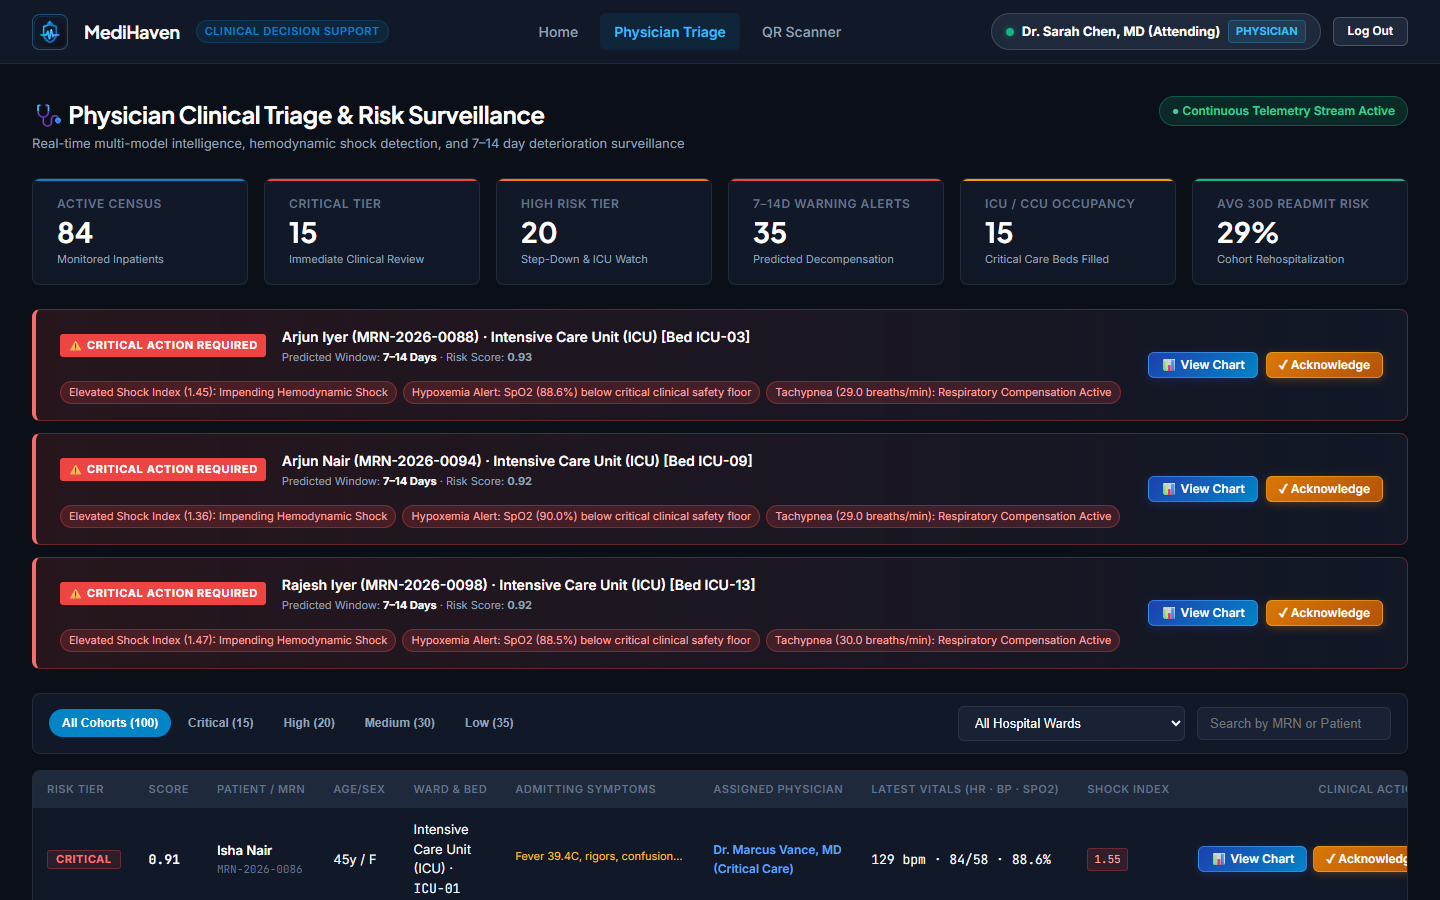
\includegraphics[width=\linewidth]{figures/screenshots/03_triage_dashboard.png}\\[-1pt]
{\footnotesize (a) Triage dashboard: KPIs, alert feed, roster}
\end{minipage}\hfill
\begin{minipage}{0.495\linewidth}\centering
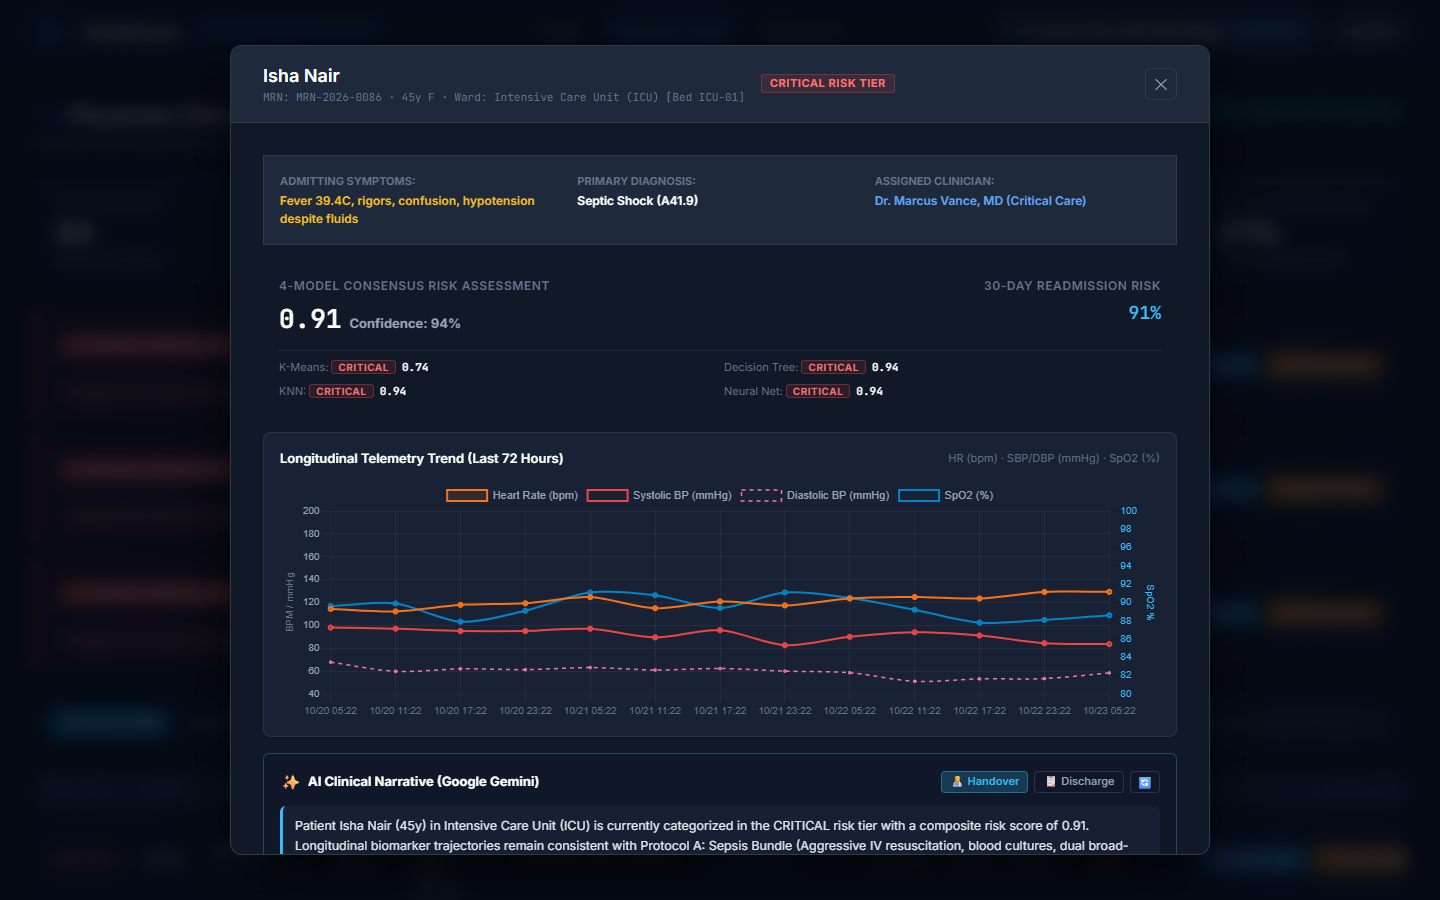
\includegraphics[width=\linewidth]{figures/screenshots/04_patient_chart_drawer.png}\\[-1pt]
{\footnotesize (b) Patient chart: 4 model votes and 72-h vitals}
\end{minipage}
\caption{Physician portal on the synthetic cohort}
\label{fig:ss-triage}
\end{figure}

\begin{figure}[!htbp]
\centering
\begin{minipage}{0.495\linewidth}\centering
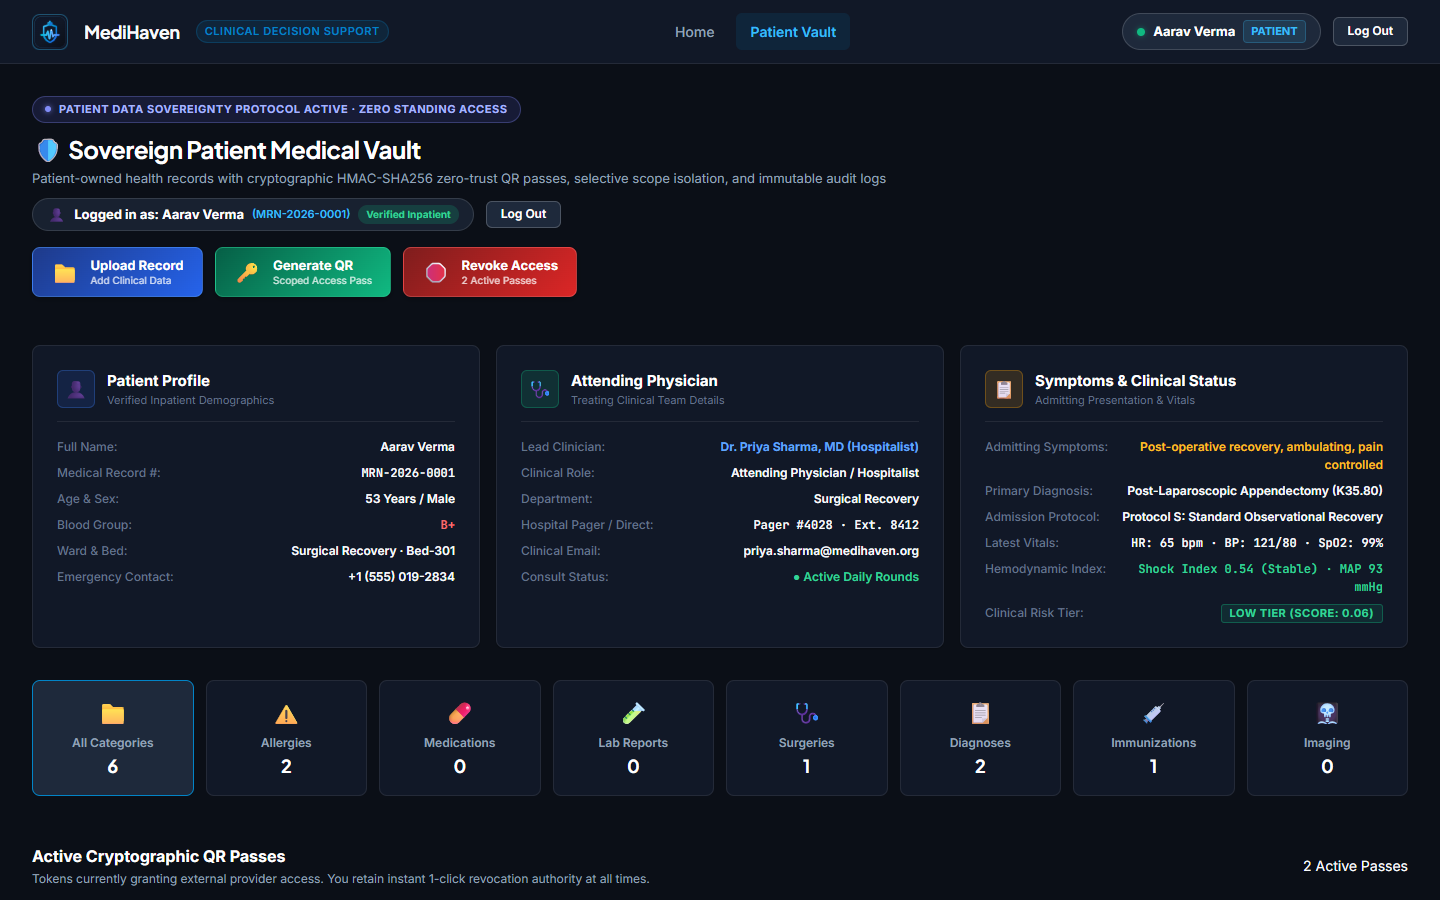
\includegraphics[width=\linewidth]{figures/screenshots/06_patient_vault.png}\\[-1pt]
{\footnotesize (a) Patient vault}
\end{minipage}\hfill
\begin{minipage}{0.495\linewidth}\centering
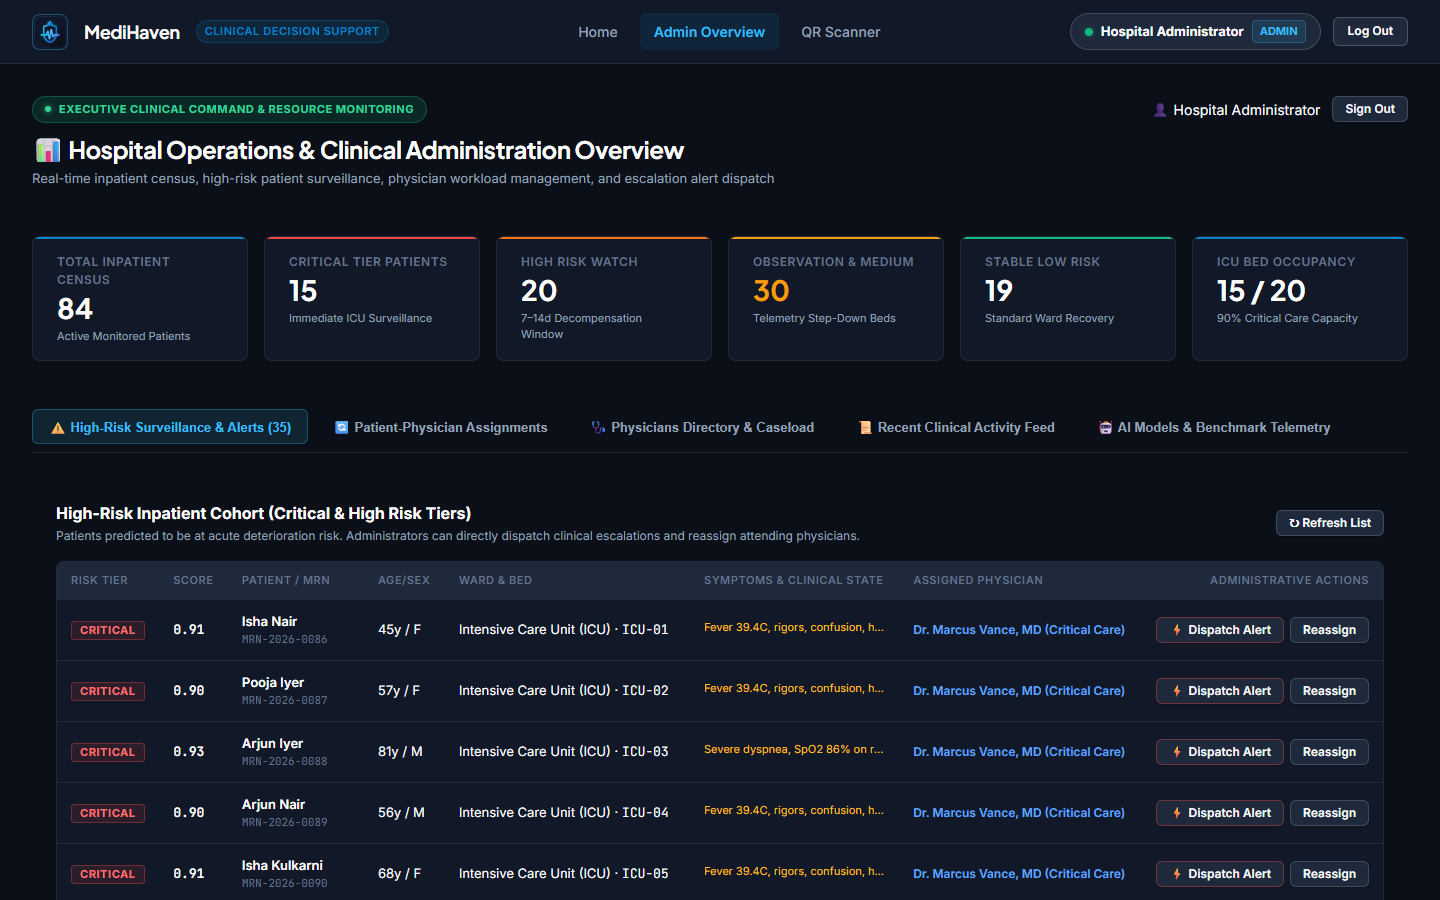
\includegraphics[width=\linewidth]{figures/screenshots/07_admin_overview.png}\\[-1pt]
{\footnotesize (b) Administrator overview}
\end{minipage}\\[6pt]
\begin{minipage}{0.55\linewidth}\centering
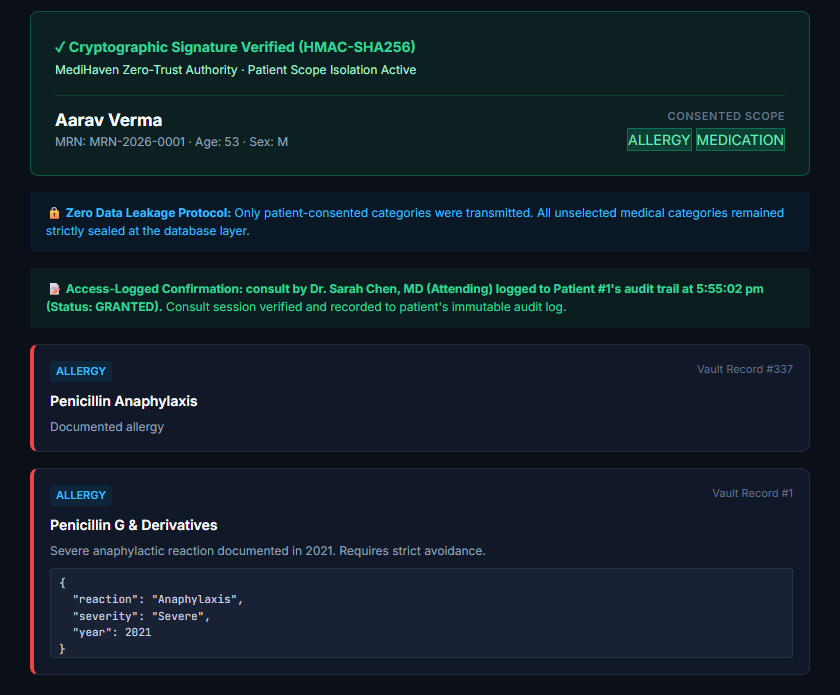
\includegraphics[width=\linewidth]{figures/screenshots/05_qr_scanner_result.png}\\[-1pt]
{\footnotesize (c) QR scanner result: only the consented categories, access logged under the signed-in clinician}
\end{minipage}
\caption{Patient, administrator and scanner portals (synthetic data)}
\label{fig:ss-portals}
\end{figure}

\begin{figure}[!htbp]
\centering
\begin{minipage}{0.495\linewidth}\centering
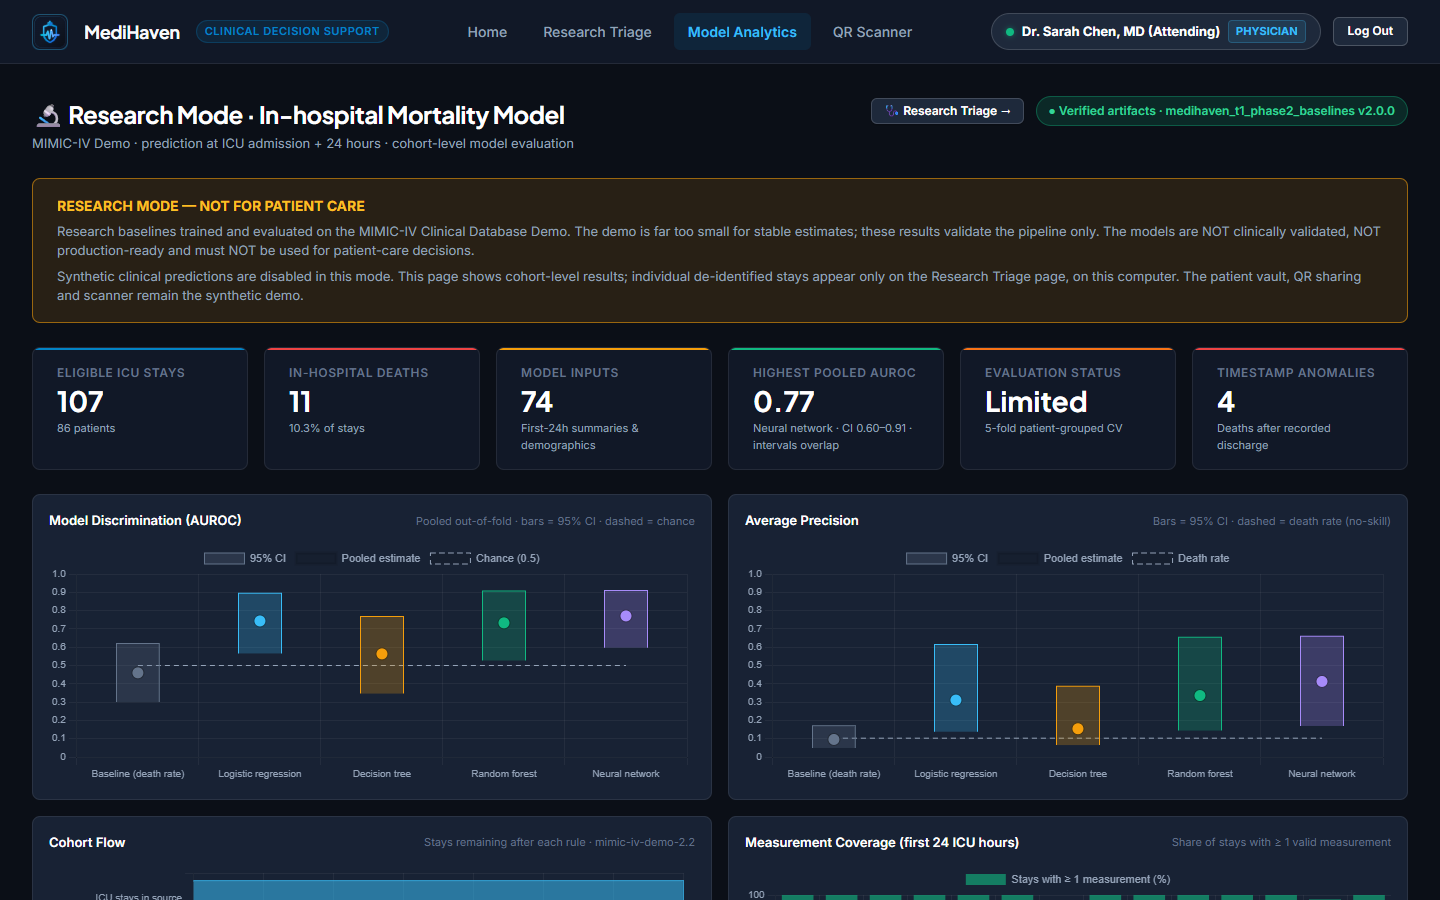
\includegraphics[width=\linewidth]{figures/screenshots/08_research_analytics_top.png}\\[-1pt]
{\footnotesize (a) Model analytics (cohort level)}
\end{minipage}\hfill
\begin{minipage}{0.495\linewidth}\centering
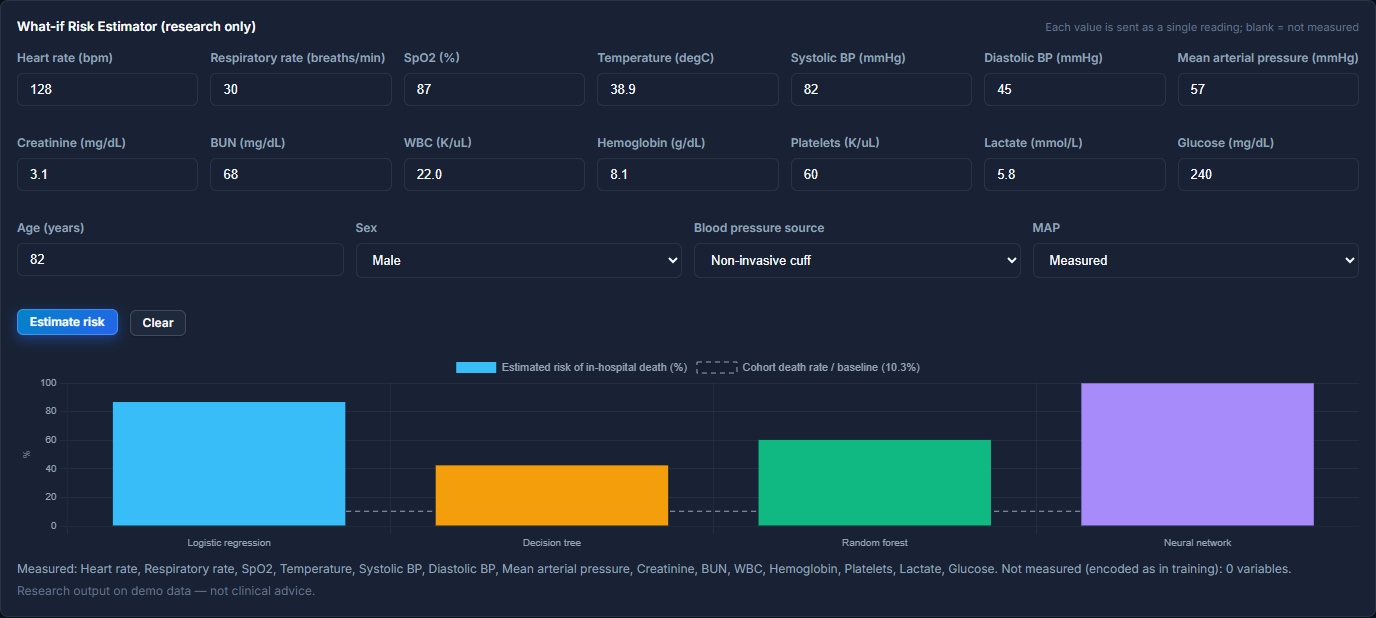
\includegraphics[width=\linewidth]{figures/screenshots/09_research_whatif.png}\\[-1pt]
{\footnotesize (b) What-if estimate for an illustrative input}
\end{minipage}\\[6pt]
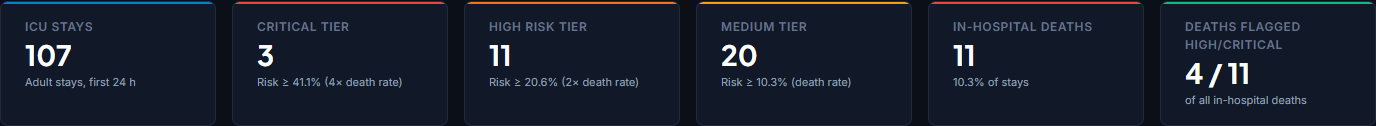
\includegraphics[width=\linewidth]{figures/screenshots/10_research_triage_kpis.png}\\[-1pt]
{\footnotesize (c) Research triage summary cards}
\caption{Research mode on the MIMIC-IV Demo (aggregate views only)}
\label{fig:ss-research}
\end{figure}

\section{Functional Results}
Each functional requirement is met by at least one passing test (Table~\ref{tab:testcases}). In the
synthetic demo every one of the 100 patients returns a tier, a score, four model votes and a non-empty
72-hour vitals series; a single-use pass grants exactly one access even under concurrent scans; research
mode refuses unsafe configuration and tampered artifacts.

\section{Performance Results}
\subsection{Server performance}
Measured server performance is reported in Chapter~\ref{ch:scal}: median prediction latency 71.9~ms for one
client, about 15 predictions/s at saturation, 268.8 simple reads/s at 16 clients, 0 errors and at most
206~MB of memory.

\subsection{Synthetic ensemble benchmark}
\label{sec:synthcaveat}
The project benchmark (\code{models_store/benchmark_report.json}, 23~October~2026) reports accuracy,
precision, recall and F1 of 1.00 on a 20-patient hold-out split and in 5-fold cross-validation, with a mean
inference latency of 24.4~ms (p95 29.5~ms). \textbf{These figures do not indicate clinical accuracy.} The
synthetic patients are generated tier by tier from tier-specific value ranges, so the tiers are nearly
separable by construction; perfect scores show only that the pipeline learns the generator.

\subsection{Research task on the MIMIC-IV Demo}
\textbf{Cohort.} Table~\ref{tab:cohort} traces the cohort (dataset v1.2.0, task v3). ``Eligible'' means
the first ICU stay of an adult admission, still alive, still in the ICU and still in hospital at the index
time (ICU admission + 24~h). The label is in-hospital death after the index time; features use only the
first 24 ICU hours. All 11 positive stays, including the 4 with a death time recorded after the discharge
time, are in the primary evaluation cohort of 107 stays; sensitivity analysis A re-scores the primary
predictions without the 4 anomalies, and B retrains without them (103 stays, 7 deaths).

\begin{table}[!htbp]
\centering
\caption{Research cohort flow (MIMIC-IV Clinical Database Demo 2.2)}
\label{tab:cohort}
\small
\begin{tabular}{@{}lr@{}}
\toprule
Step & Stays\\
\midrule
ICU stays in source & 140\\
\quad excluded: not the first ICU stay of the admission & $-12$\\
\quad excluded: died before the index time & $-1$\\
\quad excluded: left the ICU before the index time & $-20$\\
\quad excluded: ambiguous outcome fields & $0$\\
\textbf{Eligible cohort (primary evaluation)} & \textbf{107}\\
\quad positive (in-hospital death): 7 consistent + 4 flagged timestamp anomalies & 11 (10.3\,\%)\\
\quad negative & 96\\
Sensitivity cohort (anomalies removed) & 103 (7 deaths)\\
\bottomrule
\end{tabular}
\end{table}

\textbf{Baselines.} Table~\ref{tab:research} gives the pooled out-of-fold results of model set v2.0.0
(5-fold StratifiedGroupKFold by patient, seed 42; 95\,\% subject-bootstrap intervals; threshold = training
prevalence). Figure~\ref{fig:auroc} shows the AUROC intervals.

\begin{table}[!htbp]
\centering
\caption{Research baselines, primary analysis (107 stays, 11 deaths; evaluation status: limited)}
\label{tab:research}
\small
\begin{tabular}{@{}lcccc@{}}
\toprule
Model & AUROC [95\% CI] & Avg.\ precision [95\% CI] & Brier & Sens.\ / Spec.\\
\midrule
Prior-only reference & 0.46 [0.30--0.62] & 0.10 [0.05--0.17] & 0.092 & 1.00 / 0.00\\
Logistic regression & 0.74 [0.57--0.90] & 0.31 [0.14--0.62] & 0.086 & 0.73 / 0.76\\
Decision tree (smoothed) & 0.56 [0.35--0.77] & 0.15 [0.07--0.39] & 0.098 & 0.36 / 0.75\\
Random forest & 0.73 [0.53--0.91] & 0.34 [0.14--0.66] & 0.082 & 0.64 / 0.62\\
Neural network (MLP) & 0.77 [0.60--0.91] & 0.41 [0.17--0.66] & 0.087 & 0.55 / 0.85\\
\bottomrule
\end{tabular}
\end{table}

\begin{figure}[!htbp]
\centering
\begin{tikzpicture}
\begin{axis}[width=0.8\linewidth, height=50mm, ylabel={AUROC}, ymin=0.2, ymax=1.0,
  symbolic x coords={Prior,LR,DT,RF,MLP}, xtick=data, tick label style={font=\scriptsize},
  label style={font=\footnotesize}, enlarge x limits=0.15]
\addplot[only marks, mark=*, mhblue, error bars/.cd, y dir=both, y explicit]
  coordinates {(Prior,0.46) += (0,0.16) -= (0,0.16) (LR,0.74) += (0,0.16) -= (0,0.17)
               (DT,0.56) += (0,0.21) -= (0,0.21) (RF,0.73) += (0,0.18) -= (0,0.20)
               (MLP,0.77) += (0,0.14) -= (0,0.17)};
\addplot[dashed, mhred] coordinates {(Prior,0.5) (MLP,0.5)};
\end{axis}
\end{tikzpicture}
\caption{Pooled out-of-fold AUROC with 95\% subject-bootstrap intervals (Table~\ref{tab:research});
dashed line: chance (0.5)}
\label{fig:auroc}
\end{figure}

\textbf{Sensitivity analyses} (103 stays, 7 deaths). A (anomalies removed from scoring only): AUROC
LR 0.73, DT 0.52, RF 0.73, MLP 0.78. B (retrained without anomalies, folds with 1--2 deaths): LR 0.40
[0.08--0.76], DT 0.61, RF 0.71, MLP 0.39 [0.02--0.78]. \textbf{Stay-level view.} With tiers at fixed
multiples of the death rate (Medium $\ge$ 1$\times$, High $\ge$ 2$\times$, Critical $\ge$ 4$\times$
10.3\,\%), the 107 stays fall into 3 Critical, 11 High, 20 Medium and 73 Low, with 2, 2, 4 and 3 deaths
respectively; 4 of the 11 deaths were placed in High or Critical.

\section{Comparison with Existing Systems}
Compared with the systems in Table~\ref{tab:compare}, MediHaven adds patient-controlled sharing, explicit
uncertainty and fail-closed research serving, but its discrimination on real data (AUROC about 0.73--0.77
with intervals spanning roughly 0.55--0.90) is far below large-cohort models such as
\cite{rajkomar2018scalable} (0.93--0.94) and is not comparable with them, given 11 deaths and no external
validation. Bedside scores remain the only clinically validated option of those compared.

\section{Achievement of Objectives}
\begin{table}[!htbp]
\centering
\caption{Objectives and supporting evidence}
\label{tab:objectives}
\small
\begin{tabularx}{\textwidth}{@{}lYl@{}}
\toprule
Objective & Evidence & Status\\
\midrule
O1 portals and API & 44 routes; RBAC tests; Figures~\ref{fig:ss-triage}--\ref{fig:ss-portals} & achieved\\
O2 explainable ensemble & votes, rule path, KNN cases; model tests; Figure~\ref{fig:ss-triage}(b) & achieved\\
O3 secure vault and QR & scope, expiry, atomic quota, audit; TC-08 to TC-11 & achieved\\
O4 research task and evaluation & Tables~\ref{tab:cohort}--\ref{tab:research} & achieved (pipeline), performance not established\\
O5 verified research serving & hash verification, OOF reproduction; TC-14, TC-15 & achieved\\
O6 data protection & security tests; Section~\ref{sec:secdesign} & achieved for the prototype scope\\
O7 testing and measurement & 354 passing tests; Chapter~\ref{ch:scal} & achieved\\
\bottomrule
\end{tabularx}
\end{table}

\section{Discussion of Findings}
The contrast between perfect synthetic scores and modest, uncertain real-data scores is the central
finding: model quality claims depend on the data, and synthetic benchmarks validate pipelines, not
medicine. On the real cohort, the learned models beat the prior-only reference in the primary analysis,
but their intervals overlap heavily, the rankings change between analyses, and sensitivity analysis B
shows that logistic regression and the MLP collapse when only 7 deaths remain. The four timestamp anomalies
are 4 of 11 positives, so the labelling rule materially affects results. The smoothed decision tree trades
discrimination for interpretability and never outputs 0\,\% or 100\,\%.

\section{Practical Applicability}
MediHaven is suitable for teaching, demonstrations and prototyping user interfaces and data-protection
patterns. It must not be used for diagnosis, treatment or any other patient-care decision. Larger,
multi-site, credentialed data, calibration analysis, prospective evaluation and regulatory review would be
required before any clinical use could be considered.

\chapter{Conclusion and Future Scope}
\label{ch:concl}

\section{Conclusion}
MediHaven integrates explainable four-model triage on synthetic inpatients, a patient-controlled medical
vault with signed, scoped and auditable QR passes, and an opt-in research mode that rebuilds an
in-hospital-mortality task from the MIMIC-IV Clinical Database Demo and evaluates baselines with
patient-grouped cross-validation. The system is layered, tested (354 passing tests), measured under load
and hardened for deployment of the synthetic demo, while research mode stays on the researcher's machine.

\section{Achievement of Objectives}
All seven objectives were achieved as engineering deliverables (Table~\ref{tab:objectives}). Objective~O4
was achieved as a validated pipeline; clinically meaningful model performance was \emph{not} established and
was never an achievable aim on a 107-stay demo cohort with 11 deaths.

\section{Major Engineering Contributions}
A fail-closed research path (secret, bind-address and artifact-hash checks; no external AI); out-of-fold
stay-level scores that must reproduce the verified run before being served; explicit handling of outcome
timestamp anomalies; an atomic, race-free pass quota; leakage controls on time windows and feature
provenance; and measured performance with an identified CPU-bound prediction bottleneck.

\section{Current Limitations}
Synthetic data cannot show clinical validity; the real cohort is tiny and single-centre, results are
unstable across sensitivity analyses, and calibration is unassessed; the design is single-instance;
the vault stores document references, not files; no browser end-to-end or penetration tests exist; and
the demo accounts must be replaced in any deployment.

\section{Future Enhancements}
The following are future work, not implemented features: evaluation on credentialed full MIMIC-IV with
temporal or external validation and calibration analysis; per-patient feature caching and process-based
inference workers; a shared store (e.g.\ PostgreSQL and Redis) for multi-instance deployment; real,
virus-scanned document uploads; browser end-to-end and accessibility tests; and an independent security
review.

\section{Lessons Learned}
Leakage hides in timestamps; small cohorts demand intervals and sensitivity analyses rather than single
numbers; synthetic perfection is a warning sign, not a result; security defects (races, trusted client
input, plain-text secrets) are found by deliberate review and fixed with regression tests; and frequent,
reviewed commits through pull requests kept a three-person team's work integrated.

% Sections required by the SPIT template (synopsis.tex): "Research Paper" and "Plagiarism Report".
% No paper or plagiarism report was supplied; nothing here may be replaced by an invented document.
\chapter*{Research Paper and Plagiarism Report}
\addcontentsline{toc}{chapter}{Research Paper and Plagiarism Report}
\section*{Research Paper}
\noindent\missing{No research paper has been submitted or accepted for this project. If a paper is written,
insert it here with its plagiarism report and, if accepted, the acceptance receipt, as the template requires.}

\section*{Plagiarism Report}
\noindent\missing{The institutional plagiarism report for this document has not been supplied. Insert the
genuine report here (for example as \texttt{figures/plagiarism\_report.pdf} with \texttt{\textbackslash
includegraphics}) once it has been generated. No similarity score is stated or implied by this placeholder.}


% ---------------- References ------------------------------------------------
\clearpage
\phantomsection
\addcontentsline{toc}{chapter}{References}
\bibliographystyle{IEEEtran}
{\small\bibliography{bibliography}}

% ---------------- Appendix --------------------------------------------------
\appendix
\chapter{Reproducibility and API Summary}
\label{app:repro}

\section*{Commands (Windows PowerShell, repository root)}
\begin{small}
\begin{tabular}{@{}p{50mm}p{110mm}@{}}
Install & \texttt{.\textbackslash.venv\textbackslash Scripts\textbackslash python.exe -m pip install -r requirements-dev.txt}\\
Synthetic demo & \texttt{.\textbackslash.venv\textbackslash Scripts\textbackslash python.exe run\_demo.py}\\
Tests & \texttt{.\textbackslash.venv\textbackslash Scripts\textbackslash python.exe -m pytest tests/ -q -p no:cacheprovider}\\
Research dataset & \texttt{python -m src.tasks.build\_mimic\_t1 --mimic-dir <demo> --output-dir <out>}\\
Research training & \texttt{python -m src.training.train\_mimic\_t1 --research-dir <out>}\\
Research mode & \texttt{\$env:DATA\_MODE="mimic"; \$env:MIMIC\_OUTPUT\_DIR="<out>"; python run\_demo.py}\\
Production & \texttt{waitress-serve --host=0.0.0.0 --port=8000 wsgi:app} (see \texttt{docs/deployment.md})\\
Load test & \texttt{python appendices/perf\_measure.py} (this package)\\
\end{tabular}
\end{small}

\section*{API routes (44)}
\begin{footnotesize}
\begin{tabularx}{\textwidth}{@{}lY@{}}
\toprule
Group & Routes\\
\midrule
Pages & \texttt{/}, \texttt{/login}, \texttt{/logout}, \texttt{/dashboard}, \texttt{/vault}, \texttt{/scanner}, \texttt{/admin}, \texttt{/research}, \texttt{/favicon.ico}\\
Auth & \texttt{POST /api/auth/login}, \texttt{/api/auth/logout}, \texttt{GET /api/auth/me}, \texttt{GET /api/health}\\
Patients & \texttt{GET|POST /api/patients}, \texttt{GET /api/patients/<id>}, \texttt{/vitals}, \texttt{/labs}, \texttt{/predict}, \texttt{/similar}, \texttt{/clinical-narrative}, \texttt{POST /reassign}, \texttt{GET /api/patients/physicians}\\
Dashboard \& alerts & \texttt{GET /api/dashboard/summary}, \texttt{GET /api/alerts}, \texttt{POST /api/alerts/<id>/acknowledge}, \texttt{POST /api/alerts/dispatch}, \texttt{GET /api/alerts/activity}\\
Admin & \texttt{GET /api/admin/models}, \texttt{POST /api/admin/gemini/synthesize}\\
Vault & \texttt{GET /api/vault/<id>}, \texttt{/access-log}, \texttt{/active-tokens}, \texttt{POST /api/vault/upload}, \texttt{/share}, \texttt{/<id>/share}, \texttt{/access}, \texttt{/revoke/<token>}\\
Research & \texttt{GET /api/research/status}, \texttt{/model-card}, \texttt{/dashboard}, \texttt{/stays}, \texttt{/stays/<n>}, \texttt{POST /api/research/predict}\\
\bottomrule
\end{tabularx}
\end{footnotesize}


% ---------------- Final page: NIL AI content declaration --------------------
% Must remain the very last page of the report. See README.md / MISSING_INFORMATION.md.
% ============================================================================
% FINAL PAGE: NIL AI content declaration / detection image.
% The genuine official image was NOT found in the supplied materials (guidelines DOCX, template ZIP,
% repository). Do not substitute any generated or illustrative image.
% To complete the report: save the genuine image as  figures/nil_ai_declaration.png  (or .pdf / .jpg,
% then update NILImageFile below) and rebuild. The page then shows the image instead of the placeholder.
% Nothing may follow this page.
% ============================================================================
\newcommand{\NILImageFile}{figures/nil_ai_declaration.png}
\clearpage
\thispagestyle{empty}
\phantomsection
\addcontentsline{toc}{chapter}{NIL AI Content Declaration}
\begin{center}
{\large\textbf{NIL AI Content Declaration}}
\end{center}
\vspace{0.5cm}
\IfFileExists{\NILImageFile}{%
  \begin{center}
  \includegraphics[width=\textwidth,height=0.78\textheight,keepaspectratio]{\NILImageFile}
  \end{center}
}{%
  \begin{center}
  \fbox{\begin{minipage}{0.86\textwidth}
  \vspace{0.6cm}
  \centering
  {\large\textcolor{red}{\textbf{PLACEHOLDER --- GENUINE NIL AI CONTENT IMAGE REQUIRED}}}\\[0.6cm]
  \raggedright
  The official NIL AI content declaration/detection image was not present in the supplied materials
  (report guidelines, report template or project repository). It has deliberately \textbf{not} been
  recreated or simulated.\\[0.3cm]
  To complete this page, save the genuine image issued for this report as:\\[0.15cm]
  \centering\texttt{figures/nil\_ai\_declaration.png}\\[0.25cm]
  \raggedright
  and rebuild the report (\texttt{tectonic main.tex}). The image then replaces this notice
  automatically, and this page remains the last page of the report.
  \vspace{0.6cm}
  \end{minipage}}
  \end{center}
}


\end{document}
